
\documentclass{article} % For LaTeX2e
\usepackage{iclr2027_conference,times}

% Optional math commands from https://github.com/goodfeli/dlbook_notation.
%%%%% NEW MATH DEFINITIONS %%%%%

\usepackage{amsmath,amsfonts,bm}

% Mark sections of captions for referring to divisions of figures
\newcommand{\figleft}{{\em (Left)}}
\newcommand{\figcenter}{{\em (Center)}}
\newcommand{\figright}{{\em (Right)}}
\newcommand{\figtop}{{\em (Top)}}
\newcommand{\figbottom}{{\em (Bottom)}}
\newcommand{\captiona}{{\em (a)}}
\newcommand{\captionb}{{\em (b)}}
\newcommand{\captionc}{{\em (c)}}
\newcommand{\captiond}{{\em (d)}}

% Highlight a newly defined term
\newcommand{\newterm}[1]{{\bf #1}}


% Figure reference, lower-case.
\def\figref#1{figure~\ref{#1}}
% Figure reference, capital. For start of sentence
\def\Figref#1{Figure~\ref{#1}}
\def\twofigref#1#2{figures \ref{#1} and \ref{#2}}
\def\quadfigref#1#2#3#4{figures \ref{#1}, \ref{#2}, \ref{#3} and \ref{#4}}
% Section reference, lower-case.
\def\secref#1{section~\ref{#1}}
% Section reference, capital.
\def\Secref#1{Section~\ref{#1}}
% Reference to two sections.
\def\twosecrefs#1#2{sections \ref{#1} and \ref{#2}}
% Reference to three sections.
\def\secrefs#1#2#3{sections \ref{#1}, \ref{#2} and \ref{#3}}
% Reference to an equation, lower-case.
\def\eqref#1{equation~\ref{#1}}
% Reference to an equation, upper case
\def\Eqref#1{Equation~\ref{#1}}
% A raw reference to an equation---avoid using if possible
\def\plaineqref#1{\ref{#1}}
% Reference to a chapter, lower-case.
\def\chapref#1{chapter~\ref{#1}}
% Reference to an equation, upper case.
\def\Chapref#1{Chapter~\ref{#1}}
% Reference to a range of chapters
\def\rangechapref#1#2{chapters\ref{#1}--\ref{#2}}
% Reference to an algorithm, lower-case.
\def\algref#1{algorithm~\ref{#1}}
% Reference to an algorithm, upper case.
\def\Algref#1{Algorithm~\ref{#1}}
\def\twoalgref#1#2{algorithms \ref{#1} and \ref{#2}}
\def\Twoalgref#1#2{Algorithms \ref{#1} and \ref{#2}}
% Reference to a part, lower case
\def\partref#1{part~\ref{#1}}
% Reference to a part, upper case
\def\Partref#1{Part~\ref{#1}}
\def\twopartref#1#2{parts \ref{#1} and \ref{#2}}

\def\ceil#1{\lceil #1 \rceil}
\def\floor#1{\lfloor #1 \rfloor}
\def\1{\bm{1}}
\newcommand{\train}{\mathcal{D}}
\newcommand{\valid}{\mathcal{D_{\mathrm{valid}}}}
\newcommand{\test}{\mathcal{D_{\mathrm{test}}}}

\def\eps{{\epsilon}}


% Random variables
\def\reta{{\textnormal{$\eta$}}}
\def\ra{{\textnormal{a}}}
\def\rb{{\textnormal{b}}}
\def\rc{{\textnormal{c}}}
\def\rd{{\textnormal{d}}}
\def\re{{\textnormal{e}}}
\def\rf{{\textnormal{f}}}
\def\rg{{\textnormal{g}}}
\def\rh{{\textnormal{h}}}
\def\ri{{\textnormal{i}}}
\def\rj{{\textnormal{j}}}
\def\rk{{\textnormal{k}}}
\def\rl{{\textnormal{l}}}
% rm is already a command, just don't name any random variables m
\def\rn{{\textnormal{n}}}
\def\ro{{\textnormal{o}}}
\def\rp{{\textnormal{p}}}
\def\rq{{\textnormal{q}}}
\def\rr{{\textnormal{r}}}
\def\rs{{\textnormal{s}}}
\def\rt{{\textnormal{t}}}
\def\ru{{\textnormal{u}}}
\def\rv{{\textnormal{v}}}
\def\rw{{\textnormal{w}}}
\def\rx{{\textnormal{x}}}
\def\ry{{\textnormal{y}}}
\def\rz{{\textnormal{z}}}

% Random vectors
\def\rvepsilon{{\mathbf{\epsilon}}}
\def\rvtheta{{\mathbf{\theta}}}
\def\rva{{\mathbf{a}}}
\def\rvb{{\mathbf{b}}}
\def\rvc{{\mathbf{c}}}
\def\rvd{{\mathbf{d}}}
\def\rve{{\mathbf{e}}}
\def\rvf{{\mathbf{f}}}
\def\rvg{{\mathbf{g}}}
\def\rvh{{\mathbf{h}}}
\def\rvu{{\mathbf{i}}}
\def\rvj{{\mathbf{j}}}
\def\rvk{{\mathbf{k}}}
\def\rvl{{\mathbf{l}}}
\def\rvm{{\mathbf{m}}}
\def\rvn{{\mathbf{n}}}
\def\rvo{{\mathbf{o}}}
\def\rvp{{\mathbf{p}}}
\def\rvq{{\mathbf{q}}}
\def\rvr{{\mathbf{r}}}
\def\rvs{{\mathbf{s}}}
\def\rvt{{\mathbf{t}}}
\def\rvu{{\mathbf{u}}}
\def\rvv{{\mathbf{v}}}
\def\rvw{{\mathbf{w}}}
\def\rvx{{\mathbf{x}}}
\def\rvy{{\mathbf{y}}}
\def\rvz{{\mathbf{z}}}

% Elements of random vectors
\def\erva{{\textnormal{a}}}
\def\ervb{{\textnormal{b}}}
\def\ervc{{\textnormal{c}}}
\def\ervd{{\textnormal{d}}}
\def\erve{{\textnormal{e}}}
\def\ervf{{\textnormal{f}}}
\def\ervg{{\textnormal{g}}}
\def\ervh{{\textnormal{h}}}
\def\ervi{{\textnormal{i}}}
\def\ervj{{\textnormal{j}}}
\def\ervk{{\textnormal{k}}}
\def\ervl{{\textnormal{l}}}
\def\ervm{{\textnormal{m}}}
\def\ervn{{\textnormal{n}}}
\def\ervo{{\textnormal{o}}}
\def\ervp{{\textnormal{p}}}
\def\ervq{{\textnormal{q}}}
\def\ervr{{\textnormal{r}}}
\def\ervs{{\textnormal{s}}}
\def\ervt{{\textnormal{t}}}
\def\ervu{{\textnormal{u}}}
\def\ervv{{\textnormal{v}}}
\def\ervw{{\textnormal{w}}}
\def\ervx{{\textnormal{x}}}
\def\ervy{{\textnormal{y}}}
\def\ervz{{\textnormal{z}}}

% Random matrices
\def\rmA{{\mathbf{A}}}
\def\rmB{{\mathbf{B}}}
\def\rmC{{\mathbf{C}}}
\def\rmD{{\mathbf{D}}}
\def\rmE{{\mathbf{E}}}
\def\rmF{{\mathbf{F}}}
\def\rmG{{\mathbf{G}}}
\def\rmH{{\mathbf{H}}}
\def\rmI{{\mathbf{I}}}
\def\rmJ{{\mathbf{J}}}
\def\rmK{{\mathbf{K}}}
\def\rmL{{\mathbf{L}}}
\def\rmM{{\mathbf{M}}}
\def\rmN{{\mathbf{N}}}
\def\rmO{{\mathbf{O}}}
\def\rmP{{\mathbf{P}}}
\def\rmQ{{\mathbf{Q}}}
\def\rmR{{\mathbf{R}}}
\def\rmS{{\mathbf{S}}}
\def\rmT{{\mathbf{T}}}
\def\rmU{{\mathbf{U}}}
\def\rmV{{\mathbf{V}}}
\def\rmW{{\mathbf{W}}}
\def\rmX{{\mathbf{X}}}
\def\rmY{{\mathbf{Y}}}
\def\rmZ{{\mathbf{Z}}}

% Elements of random matrices
\def\ermA{{\textnormal{A}}}
\def\ermB{{\textnormal{B}}}
\def\ermC{{\textnormal{C}}}
\def\ermD{{\textnormal{D}}}
\def\ermE{{\textnormal{E}}}
\def\ermF{{\textnormal{F}}}
\def\ermG{{\textnormal{G}}}
\def\ermH{{\textnormal{H}}}
\def\ermI{{\textnormal{I}}}
\def\ermJ{{\textnormal{J}}}
\def\ermK{{\textnormal{K}}}
\def\ermL{{\textnormal{L}}}
\def\ermM{{\textnormal{M}}}
\def\ermN{{\textnormal{N}}}
\def\ermO{{\textnormal{O}}}
\def\ermP{{\textnormal{P}}}
\def\ermQ{{\textnormal{Q}}}
\def\ermR{{\textnormal{R}}}
\def\ermS{{\textnormal{S}}}
\def\ermT{{\textnormal{T}}}
\def\ermU{{\textnormal{U}}}
\def\ermV{{\textnormal{V}}}
\def\ermW{{\textnormal{W}}}
\def\ermX{{\textnormal{X}}}
\def\ermY{{\textnormal{Y}}}
\def\ermZ{{\textnormal{Z}}}

% Vectors
\def\vzero{{\bm{0}}}
\def\vone{{\bm{1}}}
\def\vmu{{\bm{\mu}}}
\def\vtheta{{\bm{\theta}}}
\def\va{{\bm{a}}}
\def\vb{{\bm{b}}}
\def\vc{{\bm{c}}}
\def\vd{{\bm{d}}}
\def\ve{{\bm{e}}}
\def\vf{{\bm{f}}}
\def\vg{{\bm{g}}}
\def\vh{{\bm{h}}}
\def\vi{{\bm{i}}}
\def\vj{{\bm{j}}}
\def\vk{{\bm{k}}}
\def\vl{{\bm{l}}}
\def\vm{{\bm{m}}}
\def\vn{{\bm{n}}}
\def\vo{{\bm{o}}}
\def\vp{{\bm{p}}}
\def\vq{{\bm{q}}}
\def\vr{{\bm{r}}}
\def\vs{{\bm{s}}}
\def\vt{{\bm{t}}}
\def\vu{{\bm{u}}}
\def\vv{{\bm{v}}}
\def\vw{{\bm{w}}}
\def\vx{{\bm{x}}}
\def\vy{{\bm{y}}}
\def\vz{{\bm{z}}}

% Elements of vectors
\def\evalpha{{\alpha}}
\def\evbeta{{\beta}}
\def\evepsilon{{\epsilon}}
\def\evlambda{{\lambda}}
\def\evomega{{\omega}}
\def\evmu{{\mu}}
\def\evpsi{{\psi}}
\def\evsigma{{\sigma}}
\def\evtheta{{\theta}}
\def\eva{{a}}
\def\evb{{b}}
\def\evc{{c}}
\def\evd{{d}}
\def\eve{{e}}
\def\evf{{f}}
\def\evg{{g}}
\def\evh{{h}}
\def\evi{{i}}
\def\evj{{j}}
\def\evk{{k}}
\def\evl{{l}}
\def\evm{{m}}
\def\evn{{n}}
\def\evo{{o}}
\def\evp{{p}}
\def\evq{{q}}
\def\evr{{r}}
\def\evs{{s}}
\def\evt{{t}}
\def\evu{{u}}
\def\evv{{v}}
\def\evw{{w}}
\def\evx{{x}}
\def\evy{{y}}
\def\evz{{z}}

% Matrix
\def\mA{{\bm{A}}}
\def\mB{{\bm{B}}}
\def\mC{{\bm{C}}}
\def\mD{{\bm{D}}}
\def\mE{{\bm{E}}}
\def\mF{{\bm{F}}}
\def\mG{{\bm{G}}}
\def\mH{{\bm{H}}}
\def\mI{{\bm{I}}}
\def\mJ{{\bm{J}}}
\def\mK{{\bm{K}}}
\def\mL{{\bm{L}}}
\def\mM{{\bm{M}}}
\def\mN{{\bm{N}}}
\def\mO{{\bm{O}}}
\def\mP{{\bm{P}}}
\def\mQ{{\bm{Q}}}
\def\mR{{\bm{R}}}
\def\mS{{\bm{S}}}
\def\mT{{\bm{T}}}
\def\mU{{\bm{U}}}
\def\mV{{\bm{V}}}
\def\mW{{\bm{W}}}
\def\mX{{\bm{X}}}
\def\mY{{\bm{Y}}}
\def\mZ{{\bm{Z}}}
\def\mBeta{{\bm{\beta}}}
\def\mPhi{{\bm{\Phi}}}
\def\mLambda{{\bm{\Lambda}}}
\def\mSigma{{\bm{\Sigma}}}

% Tensor
\DeclareMathAlphabet{\mathsfit}{\encodingdefault}{\sfdefault}{m}{sl}
\SetMathAlphabet{\mathsfit}{bold}{\encodingdefault}{\sfdefault}{bx}{n}
\newcommand{\tens}[1]{\bm{\mathsfit{#1}}}
\def\tA{{\tens{A}}}
\def\tB{{\tens{B}}}
\def\tC{{\tens{C}}}
\def\tD{{\tens{D}}}
\def\tE{{\tens{E}}}
\def\tF{{\tens{F}}}
\def\tG{{\tens{G}}}
\def\tH{{\tens{H}}}
\def\tI{{\tens{I}}}
\def\tJ{{\tens{J}}}
\def\tK{{\tens{K}}}
\def\tL{{\tens{L}}}
\def\tM{{\tens{M}}}
\def\tN{{\tens{N}}}
\def\tO{{\tens{O}}}
\def\tP{{\tens{P}}}
\def\tQ{{\tens{Q}}}
\def\tR{{\tens{R}}}
\def\tS{{\tens{S}}}
\def\tT{{\tens{T}}}
\def\tU{{\tens{U}}}
\def\tV{{\tens{V}}}
\def\tW{{\tens{W}}}
\def\tX{{\tens{X}}}
\def\tY{{\tens{Y}}}
\def\tZ{{\tens{Z}}}


% Graph
\def\gA{{\mathcal{A}}}
\def\gB{{\mathcal{B}}}
\def\gC{{\mathcal{C}}}
\def\gD{{\mathcal{D}}}
\def\gE{{\mathcal{E}}}
\def\gF{{\mathcal{F}}}
\def\gG{{\mathcal{G}}}
\def\gH{{\mathcal{H}}}
\def\gI{{\mathcal{I}}}
\def\gJ{{\mathcal{J}}}
\def\gK{{\mathcal{K}}}
\def\gL{{\mathcal{L}}}
\def\gM{{\mathcal{M}}}
\def\gN{{\mathcal{N}}}
\def\gO{{\mathcal{O}}}
\def\gP{{\mathcal{P}}}
\def\gQ{{\mathcal{Q}}}
\def\gR{{\mathcal{R}}}
\def\gS{{\mathcal{S}}}
\def\gT{{\mathcal{T}}}
\def\gU{{\mathcal{U}}}
\def\gV{{\mathcal{V}}}
\def\gW{{\mathcal{W}}}
\def\gX{{\mathcal{X}}}
\def\gY{{\mathcal{Y}}}
\def\gZ{{\mathcal{Z}}}

% Sets
\def\sA{{\mathbb{A}}}
\def\sB{{\mathbb{B}}}
\def\sC{{\mathbb{C}}}
\def\sD{{\mathbb{D}}}
% Don't use a set called E, because this would be the same as our symbol
% for expectation.
\def\sF{{\mathbb{F}}}
\def\sG{{\mathbb{G}}}
\def\sH{{\mathbb{H}}}
\def\sI{{\mathbb{I}}}
\def\sJ{{\mathbb{J}}}
\def\sK{{\mathbb{K}}}
\def\sL{{\mathbb{L}}}
\def\sM{{\mathbb{M}}}
\def\sN{{\mathbb{N}}}
\def\sO{{\mathbb{O}}}
\def\sP{{\mathbb{P}}}
\def\sQ{{\mathbb{Q}}}
\def\sR{{\mathbb{R}}}
\def\sS{{\mathbb{S}}}
\def\sT{{\mathbb{T}}}
\def\sU{{\mathbb{U}}}
\def\sV{{\mathbb{V}}}
\def\sW{{\mathbb{W}}}
\def\sX{{\mathbb{X}}}
\def\sY{{\mathbb{Y}}}
\def\sZ{{\mathbb{Z}}}

% Entries of a matrix
\def\emLambda{{\Lambda}}
\def\emA{{A}}
\def\emB{{B}}
\def\emC{{C}}
\def\emD{{D}}
\def\emE{{E}}
\def\emF{{F}}
\def\emG{{G}}
\def\emH{{H}}
\def\emI{{I}}
\def\emJ{{J}}
\def\emK{{K}}
\def\emL{{L}}
\def\emM{{M}}
\def\emN{{N}}
\def\emO{{O}}
\def\emP{{P}}
\def\emQ{{Q}}
\def\emR{{R}}
\def\emS{{S}}
\def\emT{{T}}
\def\emU{{U}}
\def\emV{{V}}
\def\emW{{W}}
\def\emX{{X}}
\def\emY{{Y}}
\def\emZ{{Z}}
\def\emSigma{{\Sigma}}

% entries of a tensor
% Same font as tensor, without \bm wrapper
\newcommand{\etens}[1]{\mathsfit{#1}}
\def\etLambda{{\etens{\Lambda}}}
\def\etA{{\etens{A}}}
\def\etB{{\etens{B}}}
\def\etC{{\etens{C}}}
\def\etD{{\etens{D}}}
\def\etE{{\etens{E}}}
\def\etF{{\etens{F}}}
\def\etG{{\etens{G}}}
\def\etH{{\etens{H}}}
\def\etI{{\etens{I}}}
\def\etJ{{\etens{J}}}
\def\etK{{\etens{K}}}
\def\etL{{\etens{L}}}
\def\etM{{\etens{M}}}
\def\etN{{\etens{N}}}
\def\etO{{\etens{O}}}
\def\etP{{\etens{P}}}
\def\etQ{{\etens{Q}}}
\def\etR{{\etens{R}}}
\def\etS{{\etens{S}}}
\def\etT{{\etens{T}}}
\def\etU{{\etens{U}}}
\def\etV{{\etens{V}}}
\def\etW{{\etens{W}}}
\def\etX{{\etens{X}}}
\def\etY{{\etens{Y}}}
\def\etZ{{\etens{Z}}}

% The true underlying data generating distribution
\newcommand{\pdata}{p_{\rm{data}}}
% The empirical distribution defined by the training set
\newcommand{\ptrain}{\hat{p}_{\rm{data}}}
\newcommand{\Ptrain}{\hat{P}_{\rm{data}}}
% The model distribution
\newcommand{\pmodel}{p_{\rm{model}}}
\newcommand{\Pmodel}{P_{\rm{model}}}
\newcommand{\ptildemodel}{\tilde{p}_{\rm{model}}}
% Stochastic autoencoder distributions
\newcommand{\pencode}{p_{\rm{encoder}}}
\newcommand{\pdecode}{p_{\rm{decoder}}}
\newcommand{\precons}{p_{\rm{reconstruct}}}

\newcommand{\laplace}{\mathrm{Laplace}} % Laplace distribution

\newcommand{\E}{\mathbb{E}}
\newcommand{\Ls}{\mathcal{L}}
\newcommand{\R}{\mathbb{R}}
\newcommand{\emp}{\tilde{p}}
\newcommand{\lr}{\alpha}
\newcommand{\reg}{\lambda}
\newcommand{\rect}{\mathrm{rectifier}}
\newcommand{\softmax}{\mathrm{softmax}}
\newcommand{\sigmoid}{\sigma}
\newcommand{\softplus}{\zeta}
\newcommand{\KL}{D_{\mathrm{KL}}}
\newcommand{\Var}{\mathrm{Var}}
\newcommand{\standarderror}{\mathrm{SE}}
\newcommand{\Cov}{\mathrm{Cov}}
% Wolfram Mathworld says $L^2$ is for function spaces and $\ell^2$ is for vectors
% But then they seem to use $L^2$ for vectors throughout the site, and so does
% wikipedia.
\newcommand{\normlzero}{L^0}
\newcommand{\normlone}{L^1}
\newcommand{\normltwo}{L^2}
\newcommand{\normlp}{L^p}
\newcommand{\normmax}{L^\infty}

\newcommand{\parents}{Pa} % See usage in notation.tex. Chosen to match Daphne's book.

\DeclareMathOperator*{\argmax}{arg\,max}
\DeclareMathOperator*{\argmin}{arg\,min}

\DeclareMathOperator{\sign}{sign}
\DeclareMathOperator{\Tr}{Tr}
\let\ab\allowbreak


\usepackage{hyperref}
\usepackage{url}
\usepackage{graphicx}
\usepackage{wrapfig}
\usepackage{algorithm}
\usepackage{algpseudocode}
\usepackage{booktabs}
\usepackage{multirow}


\title{Physics-Informed Training at the Operator Level}

% Authors must not appear in the submitted version. They should be hidden
% as long as the \iclrfinalcopy macro remains commented out below.
% Non-anonymous submissions will be rejected without review.

\author{
Shizheng Wen\thanks{Equal contribution.} \\
ETH Zürich \\
\texttt{shizheng.wen@math.ethz.ch}
\And
Marius Zeinhofer\footnotemark[1] \\
ETH Zürich \\
\texttt{marius.zeinhofer@math.ethz.ch}
\And
Siddhartha Mishra \\
ETH Zürich \\
\texttt{siddhartha.mishra@math.ethz.ch}
}

% The \author macro works with any number of authors. There are two commands
% used to separate the names and addresses of multiple authors: \And and \AND.
%
% Using \And between authors leaves it to \LaTeX{} to determine where to break
% the lines. Using \AND forces a linebreak at that point. So, if \LaTeX{}
% puts 3 of 4 authors names on the first line, and the last on the second
% line, try using \AND instead of \And before the third author name.

\newcommand{\fix}{\marginpar{FIX}}
\newcommand{\new}{\marginpar{NEW}}

%\iclrfinalcopy % Uncomment for camera-ready version, but NOT for submission.
\begin{document}


\maketitle

\begin{abstract}
   We present an approach to train neural operators physics-informed, i.e., in a self-supervised fashion, purely relying on the governing physical equations. This enables training on infinite datasets where no sample is visited twice and removes the need to produce training data in an offline phase. While previous attempts for physics-informed training at the operator level were limited to benign problems and performed considerably worse than data-driven learning, our approach matches the gold-standard of data-driven training at a similar optimization cost. Our method is based on modifying the physics-informed loss functions to include a preconditioner such as a multigrid method to drastically reduce the ill-conditioning caused by unbounded PDE operators. We derive the improved conditioning theoretically, and illustrate the potential of the method for the Poisson, Allen-Cahn, and stationary Stokes equation, where it performs virtually identical to data-driven training at a comparable computational cost.
\end{abstract}

\section{Introduction}

% Importance of fast solutions of PDEs. A tool for this in the age of AI: neural operators
\paragraph{Neural Operators}
Despite a century of development of numerical methods, partial differential equations (PDEs) remain expensive to solve, even more so in many-query situations, such as uncertainty quantification, optimal control, and inverse problems. The development of fast PDE solution techniques, e.g., through reduced-order/surrogate models therefore is of utmost importance. In the wake of the deep learning revolution, neural operators emerged as a powerful computational tool for surrogate modeling, drastically reducing PDE solution time in many applications. Neural operators approximate maps between infinite-dimensional spaces (operators) by a neural network, and are typically trained in a supervised fashion. They hence require a dataset that is built in an offline fashion, before they can be trained, and eventually used downstream. Data generation can constitute a substantial part of the computation and engineering effort, even more so in the context of physics foundation models that are pre-trained over an array of different PDE instances.

% Declared here, after the text that fills page 1, so [t] places it at the top of page 2.
% Regenerate with
%   python experiments/graphical_abstract/plot_abstract.py \
%       --bare output/graphical_abstract/abstract_v1_65grid_omega_opt/bare.npz \
%       --mg   output/graphical_abstract/abstract_v1_65grid_omega_opt/mg.npz \
%       --out  paper/figures/graphical_abstract.png
% Authored at exactly \textwidth, so do not rescale it.
\begin{figure}[t]
   \centering
   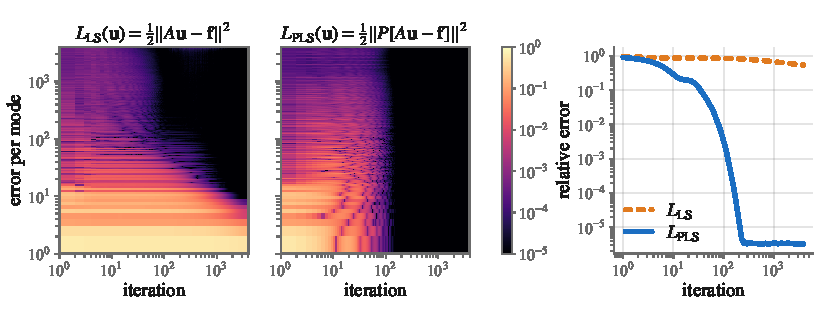
\includegraphics[width=\linewidth]{figures/graphical_abstract.pdf}
   \caption{Ill-conditioning in physics-informed learning: The figure compares Adam minimization of a linear model with and without preconditioning for a physics-informed loss originating from a Poisson problem on a $65^2$ grid. The \textbf{left} and \textbf{centre} report error in each eigenmode of $A$ along the iteration, with the smoothest mode at the bottom. The \textbf{right} figure compares the relative $L^2$ error during training.}
   \label{fig:graphical_abstract}
\end{figure}

% Physics-Informed Training: desirable but presently infeasible (prior to this work)
\paragraph{Physics-Informed Training}

Whenever the governing physics in the form of PDEs are known, neural operators can---in principle---be trained in a self-supervised fashion, relying on the physics residual or variational principles as a loss function. This approach is referred to as \emph{physics-informed neural operator training}, and a natural idea present in the community since the inceptions of neural operators []. However, the success of physics-informed training of neural operators has remained limited to benign equations and learning tasks. More often than not, purely physics-informed learning fails to converge. In fact, supervised learning with its offline data-generation pipeline remains the gold standard for almost all applications. Nevertheless, physics-informed training offers unique advantages, such as the training in the infinite data-limit, where no sample is revisited, and, of course, it removes the need of an expensive dataset generation process.

% We identify the culprit that has prevented physics-informed neural operator learning
\paragraph{Ill-Conditioning of PDE Operators}
In this manuscript, we show that the pathologies of physics-informed neural operator learning can be attributed to a single foundational property of PDE operators: PDE operators are unbounded maps, meaning they magnify their inputs without bounds, and thus lead to severe ill-conditioning in physics-informed loss functions. To make this concrete, take the derivative operator
\begin{equation}\label{eq:derivative_operator}
   \frac{d}{dx}: C^1(0,1) \subset L^2(0,1) \to L^2(0,1), \quad u \mapsto u',
\end{equation}
which amplifies oscillations: $x\mapsto \sin(\omega x)$ is bounded in $L^2(0,1)$ independent of $\omega \in \mathbb R$, but its derivative $x\mapsto \omega \cos(\omega x)$ grows without bound in $L^2(0,1)$ when $\omega \to \infty$. This phenomenon is inherent in all PDE operators. In the case of Poisson's equation, and for a linear model that is the linear combination of a given basis set $\phi_1, \dots, \phi_n$, the physics-informed least-squares loss\footnote{If the equation admits, energy formulations (variational principles) are an attractive alternative.} on a single data point $f$ takes the form
\begin{equation}\label{eq:physics_informed_ls_loss_no_precond}
   L_{\textup{LS}}(u) = \frac12 \| Au - f \|^2, \quad A_{ij} = \int_\Omega \nabla \phi_j \nabla \phi_i\,\mathrm dx,
\end{equation}
where $A\in\mathbb R^{N\times N}$ is the stiffness matrix. The condition number of $A$ scales like $h^{-2}$ for standard bases, where $h$ is the characteristic mesh-size. Conditioning thus deteriorates under mesh refinement, as higher oscillating frequencies can be resolved, the same manifestation of the unbounded nature of PDE operators stressed in \ref{eq:derivative_operator}. Note tha $\nabla^2L_{\textup{LS}} = A^2$, hence the condition number governing the convergence speed of gradient descent (GD) scales like $h^{-4}$. Figure \ref{fig:graphical_abstract} illustrates that this ill-conditioning is so severe that training with first-order methods like GD and Adam becomes infeasible already for very coarse meshes, even in the benign case of a linear ansatz (no neural network at all). In the remainder of this article, we show that precisely this ill-conditioning renders physics-informed neural operator learning infeasible.

\paragraph{Preconditioned Physics-Informed Training}

To counter the ill-conditioning of the least-squares loss \eqref{eq:physics_informed_ls_loss_no_precond}, we rely on \emph{preconditioning}---precisely the tool the numerical analysis community uses to efficiently employ iterative methods in ill-conditioned settings in classical scientific computing. Abstractly, we \emph{modify the least-squares loss} to include an invertible preconditioner $P$ and a positive definite and symmetric weighting matrix $B$
\begin{equation}\label{eq:preconditiones_least_squares_loss}
   L_{\textup{PLS}}(u) = \frac12 \| P[Au - f] \|_B^2,
\end{equation}
We stress that this construction is agnostic to the neural operator architecture employed and adds zero overhead to the inference once training finishes as it only influences the loss function. On a conceptual level, the preconditioned loss \eqref{eq:preconditiones_least_squares_loss} changes the norm in which the error is measured. For any given $P$ we can recast the 
\begin{equation*}
   L_{\textup{PLS}}(u) 
   =
   \frac12 \| P[Au - f] \|_B^2 
   =
   \frac12(PAe, PAe)_B
\end{equation*}
with the error $e=u - A^{-1}f$. This means $P$ maps $Ae$ into a different space and thereby improves conditioning, and $B$ measures the error in this space in an appropriate manner. The choice $P=A^{-1}$ and $B=I$\footnote{Or alternatively, $B=M$, where $M$ is the mass matrix.} recovers data-driven training and reduces the condition number of $\nabla^2L_{\textup{PLS}}$ to unity. In practice, this is realized through fast approximate inverses $P\approx A^{-1}$, e.g., via multigrid methods []. Note that $P\approx A^{-1}$ is not the only choice; for saddle point problems, we alternatively employ block-diagonal preconditioners. Additionally, whenever applicable, we investigate energy formulations, as these are naturally less ill-conditioned.

\subsection{Main Contributions} The main contributions are
\begin{itemize}
   \item \textbf{Efficient physics-informed neural operator training.} We demonstrate that preconditioned physics-informed neural operator training allows data-free training of neural operators at comparable cost and accuracy of the gold standard of data-driven training. Our approach vastly outperforms previous approaches and is demonstrated for the Poisson, Allen-Cahn, and Stokes equation.
   \item \textbf{Flexibility and inference speed.} Our method can be combined with any neural operator architecture and once trained, adds no additional cost to the inference.
   \item \textbf{Training at infinite data limit.} Physics-informed training allows to practically approximate the infinite data limit, where no sample is visited twice. We demonstrate empirically that this is a favorable training paradigm for neural operators.
\end{itemize}

\subsection{Related Literature}
\begin{itemize}
    \item Discussion of physics-informed training in general, in particular for PINNs and NQS.
    \item Paper of Wolfgang and Markus on preconditioning.
    \item OG paper on physics-informed neural operators.
    \item Papers on suboptimal fixes for physics-informed neural operator training.
\end{itemize}

\section{Physics-Informed Training of Neural Operators}

Our goal is to approximate an operator $\mathcal G:\mathcal F \to \mathcal U$ between function spaces $\mathcal U$ and $\mathcal F$. We aim to approximate $\mathcal G$ by a neural network $\mathcal G \approx \mathcal G_\theta$. Neural operators are a special class of neural networks well-suited to the infinite-dimensional nature of the function spaces appearing in PDE applications. However, the concrete neural network structure of $\mathcal G_\theta$ is secondary for our proposed training methodology. A simple but crucial observation we make, is that we can always write the neural operator output in the \emph{interpolated form} %I want this representation to get a name
\begin{equation}\label{eq:neural_operator_interpolated_form}
   \mathcal G_\theta(f) = \sum_{i=1}^n \mathbf{u}(\theta, f)_i \phi_i,
\end{equation}
where $\mathbf u(\theta, f)\in\mathbb R^n$ are coefficients depending on the trainable weights and the functional input $f$. The functions $\phi_1, \dots,\phi_n$ are a fixed basis and span a finite-dimensional function space $\mathcal U_h$, where $h$ denotes a characteristic mesh-size\footnote{Or more general, a quantification of how ``fine'' the space $\mathcal U_h$ is.}. Typical choices are finite element spaces, like piecewise polynomial spaces on a triangulated computational domain. It is crucial to stress that $\phi_1,\dots, \phi_n$, and thus $\mathcal U_h$ is a modeling choice, and a standard neural operator architecture will not automatically map into $\mathcal U_h$. However, we can always interpolate into $\mathcal U_h$. This is a typically sparse, non-trainable operation that adds negligible computational overhead and we will from now on assume that our neural operator is the form described in \eqref{eq:neural_operator_interpolated_form}.

\subsection{Physics-Informed Loss Functions}
For simplicity of exposition, we will work in the setting of linear PDEs that can be formulated in terms of bilinear forms, and we will restrict the discussion to learning the solution operator of such PDEs, although our experimental evaluation is broader. The operator learning problem is to find $u\in\mathcal U$ such that for given $f\in\mathcal F$ it holds
\begin{equation}\label{eq:weak_formulation}
   a(u,v) = f(v), \quad \text{for all }v\in\mathcal U.
\end{equation}
Here, $a$ is a bounded and symmetric bilinear form on $\mathcal U$, and the setting implies $\mathcal F=\mathcal U^*$. We assume all spaces to be Hilbert spaces. The solution operator is $\mathcal G:f\mapsto u$, where $u$ solves \eqref{eq:weak_formulation}. The weak equation can be written as a matrix equation, once $u$ is approximated in $\mathcal U_h$, and takes the form
\begin{equation*}
   A\mathbf u = \mathbf f, \quad \text{with }A_{ij} = a(\phi_j, \phi_i), \quad \mathbf f_i=f(\phi_i).
\end{equation*}
From this equation, we derive the single sample physics-informed loss function via a least-squares construction
\begin{equation}\label{eq:LS_loss_in_theta}
   L_{\textup{LS}}(\theta) = \frac12 \| A \mathbf u(\theta, f) - \mathbf f \|^2.
\end{equation}
For analysis purposes, we will frequently ignore the nonlinear parametrization $\mathbf u(\theta, f)$ and work in the Euclidean space of $\mathbf u\in\mathbb R^n$ directly. We indicate this by writing $L_{\textup{LS}}(u) = \frac 12 \| A\mathbf u - \mathbf f \|^2$ with the understanding that everything is in the variable $\mathbf u$.
% \begin{equation}\label{eq:LS_loss_in_u}
%    L_{\textup{LS}}(u) = \frac 12 \| A\mathbf u - \mathbf f \|^2
% \end{equation}
If $a$ is coercive and symmetric, an energy formulation is an attractive alternative to \eqref{eq:weak_formulation}. In this case, we can find the solution $u$ via a variational principle as the minimizer of the energy $\tfrac12 a(v,v)-f(v)$. The loss function to train the neural operator is, again on a single sample
\begin{equation}\label{eq:variational_loss_in_theta}
   L_{\textup{Var}}(\theta)= \frac12 \mathbf u(\theta, f)^\top A \mathbf u(\theta, f) - \mathbf f^\top \mathbf u(\theta, f).
\end{equation}


\subsection{Preconditioning} %state convergence result of GD to illustrate why ill-conditioning is relevant?
The least-square loss \ref{eq:LS_loss_in_theta}, although faithfully recovering the solution of $A\mathbf u = \mathbf f$ whenever $A$ is bijective, is unworkable in practice due to its ill-conditioning. This can be seen by computing the Hessian $\nabla_u^2 L_{\textup{LS}}=A^\top A$. In the representative scenario of the Poisson equation [], the condition number $\kappa(A^\top A)$ scales like $h^{-4}$, and makes iterative methods inefficient or, due to round-off errors, entirely useless. To counter this effect, we propose the preconditioned least-squares loss
\begin{equation}
   L_{\textup{PLS}}(u) = \frac12 \| P[A\mathbf u - \mathbf f] \|_B^2,
\end{equation}
where $P\in\mathbb R^{n\times n}$ is an invertible matrix, and $B\in\mathbb R^{n\times n}$ is symmetric and positive definite, hence induces an inner product. The choice of $P$ and $B$ is intuitively coupled: $P$ transforms the range space of $A$ thereby improving conditioning, and $B$ should induce a meaningful norm on the transformed space. To assess conditioning of $L_{\textup{PLS}}$, we compute the Hessian with respect to $\mathbf u$
\begin{equation}
   \nabla^2_u L_{\textup{PLS}}(u) = A^\top P^\top B P A.
\end{equation}
We discuss a few choices of $P$ and $A$.

\subsubsection{Approximate Inverse Preconditioners}\label{sec:approximate_inverse_preconditioner} We refer to the choice $P\approx A^{-1}$ and $B=I$ or a similarly well-conditioned matrix, like the mass matrix $M_{ij}=(\phi_i,\phi_j)_{L^2}$ as the approximate inverse setting. As proven in Lemma [] in the Appendix, this yields
\begin{equation*}
   \kappa(PA)^2 
   \approx
   \frac{\kappa(PA)^2}{\kappa(B)}
   \leq
   \kappa(A^\top P^\top B P A) 
   \leq 
   \kappa(PA)^2\kappa(B)
   \approx 
   \kappa(PA)^2
\end{equation*}
and in the case of a well conditioned matrix $B$, the conditioning is determined by the accuracy of the approximation $P\approx A^{-1}$. The approximate inverse setting is only practical when the application of $P$ is computationally efficient. For elliptic equations, multigrid methods provide such a preconditioner $P$ at the optimal complexity $\mathcal O(n)$, see [].

\subsubsection{Block-diagonal Preconditioners}\label{sec:block_diagonal_preconditioner} We assume the following block structure for $A$, $\mathbf u$ and $\mathbf f$
\begin{align*}
   A = 
   \begin{pmatrix}
      K & D^\top \\ 
      D & 0   
   \end{pmatrix},
   \quad
   \mathbf u = 
   \begin{pmatrix}
      \mathbf w \\
      \mathbf p
   \end{pmatrix},
   \quad
   \mathbf f =
   \begin{pmatrix}
      \mathbf g \\
      0
   \end{pmatrix}.
\end{align*}
We assume that $K$ is symmetric and positive definite, and that $D^\top$ is injective. In this situation the symmetric system $A$ is indefinite and invertible---a well-posed discretization of a saddle point problem, as arises from Stokes equation. The Schur complement is $S=DK^{-1}D^\top$, and the classical choice of block-diagonal preconditioner is
\begin{equation*}
   P \approx \operatorname{diag}(K^{-1}, S^{-1}),
\end{equation*}
where in applications the block inverses can frequently be handled by multigrid methods. The key property of the preconditioner is that $PA$ has exactly three eigenvalues $\{ 1, \frac{1+\sqrt 5}{2}, \frac{1-\sqrt 5}{2} \}$. However, $PA$ remains ill-conditioned in Euclidean norm as it is a non-normal matrix, and in particular, $P$ is not an approximate inverse of $A$. To leverage $P$ in the context of the least-squares loss, we use it to measure the norm of the residual (we use it as $B$ in \eqref{eq:preconditiones_least_squares_loss}), i.e., the loss becomes
\begin{equation*}
   \frac{1}{2} \| A\mathbf u - \mathbf f \|^2_P 
   =
   \frac12 \| K\mathbf w + D^\top \mathbf p - \mathbf g \|^2_{K^{-1}} + \frac12 \| D\mathbf p \|^2_{S^{-1}}.
\end{equation*}
As $A$ is symmetric, its Hessian is $APA$, and Lemma [] shows 
\begin{equation*}
   \kappa(APA) \leq \kappa(P)\left(\frac{\max|\lambda(PA)|}{\min|\lambda(PA)|}\right)^2.
\end{equation*}
Hence conditioning is governed by $\kappa(P)$, which is $\mathcal O(h^{-2})$ for the prototypical case of Stokes equation, hence ill-conditioning remains, but is drastically improved from the $\mathcal O(h^{-4})$ scaling without preconditioner. We discuss further preconditioning options with the block-diagonal preconditioner in Appendix [], but stress that all lead to worse outcomes. Finally, we mention that for Stokes equation monolithic multigrid methods exist, and these fall under the approximate inverse setting.

\subsubsection{Preconditioning Energy Formulations}
Whenever the form $a$ is symmetric and coercive, we can use the loss function $L_{\textup{Var}}(\mathbf u) = \tfrac12\mathbf u^\top A \mathbf u - \mathbf f^\top u$. Its Hessian in $\mathbf u$ is
$
   \nabla^2_u L_{\textup{Var}} = A,
$
hence its conditioning is the square root of $L_\textup{LS}$; and in the prototypical setting of the Poisson equation, it is $\mathcal O(h^{-2})$. Under the restrictive assumption that $P$ and $A$ commute and $P$ is symmetric and positive definite, we can define the preconditioned variational loss
\begin{equation*}
   L_{\textup{PVar}}(\mathbf u) = \frac12 (\mathbf u, A \mathbf u)_P - (\mathbf f, \mathbf u)_P.
\end{equation*}
The critical points $\nabla_u L_{\textup{PVar}}(\mathbf u) = 0$ are characterized by $PA\mathbf u = P\mathbf f$, and thus the minimizer of $L_\textup{Var}$ is unchanged under this transformation. The Hessian is
$
   \nabla^2_u L_{\textup{PVar}}(\mathbf u) = PA.
$
Preconditioners that commute with $A$ are e.g. polynomials in $A$ like []. In practice, we \emph{violate the requirement} $PA=AP$ and merely modify the gradient $\nabla_u L_\textup{Var}(\mathbf u) = A\mathbf u - \mathbf f$ to be $P[A\mathbf u - \mathbf f]$ in the backward pass. Empirically, the choice $P\approx A^{-1}$ via a multigrid method performs reasonable although commutativity is not exactly satisfied.

\subsubsection{Preconditioning Through Architecture Modification}
For both $L_{\textup{LS}}$ and $L_{\textup{Var}}$ we can---in principle---achieve preconditioning by a transformation with $P$: $\tilde L_\textup{LS}(\mathbf u) = L_\textup{LS}(P\mathbf u)$. This yields for $B=I$ for simplicity
\begin{equation*}
   \nabla_u^2 \tilde L_{\textup{LS}}(\mathbf u) = P^\top A^\top A P,
\end{equation*}
and similarly $\nabla_u^2 \tilde L_{\textup{Var}}(\mathbf u) = P^\top A P$. However, this construction requires $P$ to be evaluated at inference time as a part of the forward pass of the model, which is why we do not develop this idea further in this manuscript.

\section{Numerical Results}

We summarize our main experimental findings in Table~\ref{tab:summary}.

\begin{table}[t]
  \caption{Summary across the three PDE instances. Errors are relative $L^2$ on the test
  set at the best-validation checkpoint, mean $\pm$ half-range over three seeds. For Stokes each
  cell lists the velocity and pressure errors separately as $u$ / $p$, each in its own finite
  element $L^2$ norm; model selection uses their mean. Poisson and Allen--Cahn are posed on a
  uniform grid and use an FNO; Stokes is posed on an unstructured triangulation of a domain with
  a circular hole and uses the GAOT backbone of Appendix~\ref{appendix:details_stokes}, on which
  a finite-difference residual is unavailable. The last column is the wall-clock time of one
  training epoch on a single RTX 4090, in seconds.}
  \label{tab:summary}
  \centering
  \footnotesize
  \begin{tabular}{llccr r}
    \toprule
    PDE & loss & physics-informed & derivatives & rel.\ test $L^2$ & time / epoch \\
    \midrule
    \midrule
    \multirow{4}{*}{Poisson}
      & $L_\textup{PLS}$ & yes & FEM & $0.051 \pm 0.008$ & 1.2 \\
      & $L_\textup{data}$ & no & --- & $0.047 \pm 0.008$ & 1.1 \\
      & PINO & yes & FD & $0.331 \pm 0.011$ & 1.1 \\
      & PI-DeepONet & yes & AD & $0.214 \pm 0.047$ & 3.1 \\
    \midrule
    \multirow{4}{*}{Allen--Cahn}
      & $L_\textup{PLS}$ & yes & FEM & $0.032 \pm 0.003$ & 46 \\
      & $L_\textup{data}$ & no & --- & $0.020 \pm 0.002$ & 40 \\
      & PINO & yes & FD & $0.053 \pm 0.016$ & 40 \\
      & PI-DeepONet & yes & AD & $0.900 \pm 0.017$ & 8.2 \\
    \midrule
    \multirow{3}{*}{Stokes}
      & $L_\textup{PLS}$ & yes & FEM & $0.0155 \pm 0.0020$ / $0.0085 \pm 0.0004$ & 3.9 \\
      & $L_\textup{data}$ & no & --- & $0.0327 \pm 0.0015$ / $0.0179 \pm 0.0016$ & 2.9 \\
      & PI-DeepONet & yes & AD & $0.444 \pm 0.043$ / $0.351 \pm 0.012$ & 1.5 \\
    \bottomrule
  \end{tabular}
\end{table}


\subsection{Poisson Equation}
We approximate the solution operator $\mathcal G$ of the homogeneous Poisson equation
\begin{align}\label{eq:poisson_equation}
   \begin{split}
      -\Delta u &= f \quad \text{in }\Omega,
      \\
      u &= 0 \quad \text{on }\partial\Omega,
   \end{split}
\end{align}
on the domain $\Omega = [0,1]$ by a FNO $\mathcal G_\theta$. More precisely, $\mathcal G$ maps $f$ to the solution $u$ of \eqref{eq:poisson_equation}. We work on a structured tensor-product grid, and the output of the FNO is interpolated into the space $\mathcal U_h = Q_1^h$ of bilinear quadrilateral finite elements, with basis functions denoted by $\phi_1, \dots,\phi_n$. The corresponding stiffness matrix $A_{ij} = \int_\Omega \nabla \phi_j \nabla \phi_i\,\mathrm dx$ is symmetric and positive definite, which makes both the least-squares loss \ref{eq:LS_loss_in_theta} and variational loss \ref{eq:variational_loss_in_theta} available. As preconditioner $P=P_{\textup{GMG}}$, we employ single V-cycle di-adic geometric multigrid, which falls in the approximate inverse setting \ref{sec:approximate_inverse_preconditioner}. The full details are given in Appendix \ref{appendix:details_poisson}.

\subsubsection{Ill-Conditioning Prevents Physics-Informed Training}
In this experiment, we show that the ill-conditioning of the stiffness matrix $A$ is the reason physics-informed training fails without a preconditioner. To demonstrate this, we use the physics-informed least-squares loss with $B=I$ and a parametrized preconditioner
\begin{equation}
   L^t_\textup{PLS}(\mathbf u) = \frac12 \|P_t[A\mathbf u - \mathbf f] \|^2_2, \quad P_t = (1-t)I + t A^{-1}.
\end{equation}

\begin{wrapfigure}{r}{0.40\textwidth}
   \vspace{-\intextsep}
   % Authored at exactly 0.40\textwidth by
   % experiments/poisson/poisson_paper/infinite_data/plot_scaling.py, so do not rescale it.
   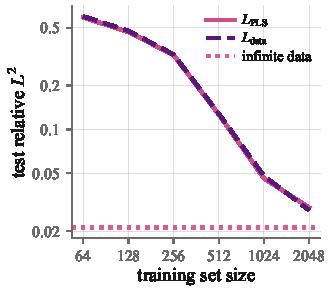
\includegraphics[width=\linewidth]{figures/infinite_data.pdf}
   \vspace{-1em}
   \caption{Test error vs.\ training set size at a fixed optimization budget for finite and infinite datasets.}
   \label{fig:data-scaling}
\end{wrapfigure}

The preconditioner $P_t$ is a convex mixing between no preconditioning $P_0=I$ and data-driven training $P_1 = A^{-1}$. This pedagogical choice is possible on a small $65\times 65$ grid, and serves to illustrate the effect of preconditioning on the training dynamics. We monitor the relative $L^2(\Omega)$ error averaged over the validation set during training for a number of $t$-values, and compare to the single di-adic V-cycle geometric multigrid preconditioner. The results are reported in Figure [], where we additionally report the condition number of the Hessian $H_t=\nabla_u^2 L_\textup{PLS}^t = AP_t^2A$. The dataset uses $K=4$.

\begin{figure}[t]
  \centering
  % Both authored at exactly 0.49\textwidth (2.695 in) by
  % experiments/poisson/sweep_blend/plot_paper.py, so do not rescale them.
  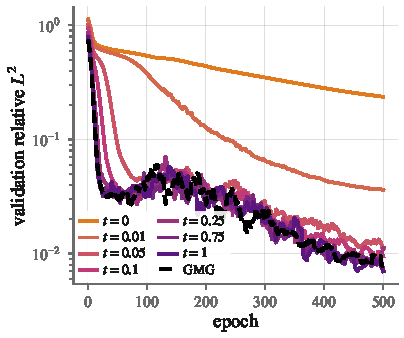
\includegraphics[width=0.49\linewidth]{figures/sweep_overlay.pdf}
  \hfill
  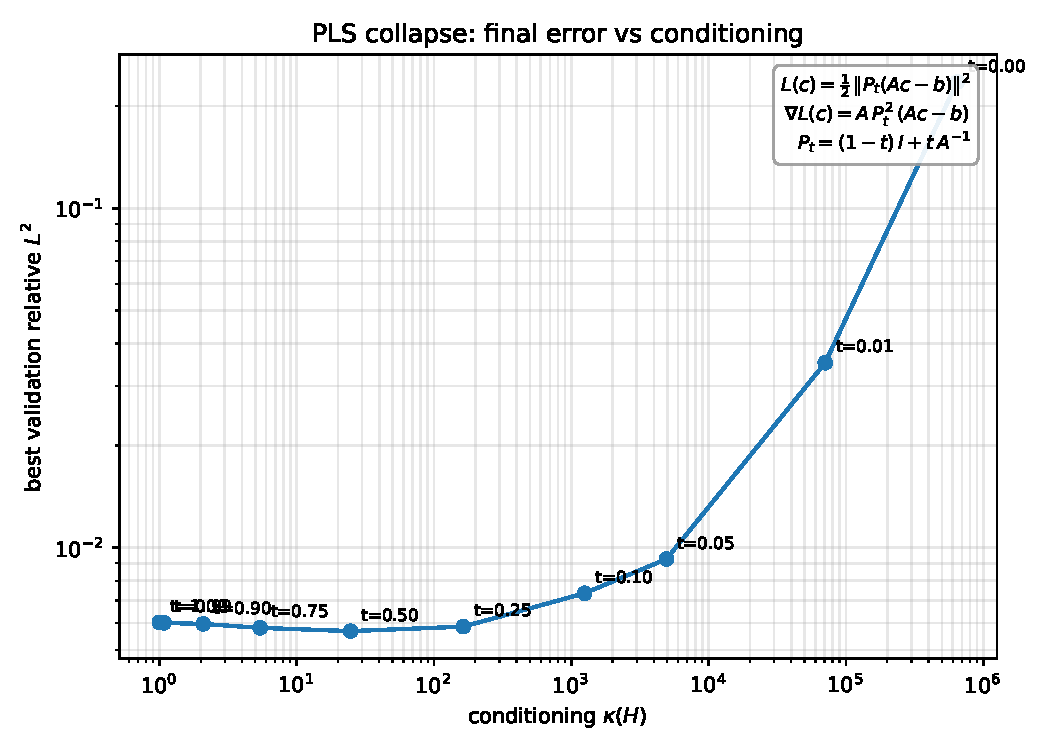
\includegraphics[width=0.49\linewidth]{figures/sweep_collapse.pdf}
  \caption{Preconditioned least-squares training for the Poisson equation. \textbf{Left:} validation relative $L^2$ vs.\ epoch as the preconditioner $P_t$ is swept from $I$ to $A^{-1}$, together with the geometric multigrid preconditioner \textbf{Right:} test error, at the best-validation checkpoint, of the $P_t$ preconditioned sweeps against the condition number $\kappa(H_t)$ of the preconditioned loss Hessian; the dashed line is the geometric multigrid preconditioner, which has no finite $\kappa(H_t)$.}
  \label{fig:pls-overlay}
\end{figure}


Figure \ref{fig:pls-overlay} shows that that preconditioning is essential to obtain efficient physics-informed training. The un-preconditioned run ($t=0$) converges to $\approx 30\%$ relative $L^2$ error after 500 epochs of training with Adam., while data-driven training ($t=1$) lands at below $1\%$ error for the same amount of training epochs. Intermediate values of $t$ interpolate the training dynamics, which leads us to conclude that ill-conditioning prevents efficient physics-informed neural operator training, and preconditioning is an effective strategy to mitigate this. This is further supported by tracking the condition numbers of $H_t$ in dependence on $t$. For $t=0$, we have $\kappa(H_t)=6.5e+05$ and of course for data-driven training it holds $\kappa(H_1)=1$. Interestingly, as visualized on the right of Figure \ref{fig:pls-overlay} below a conditioning of $approx 10^3-10^4$ (corresponding to $t\in[0.05, 0.1]$) we observe diminishing returns for making the preconditioners more accurate. We attribute this to ill-conditioning induced by the neural network parametrization, which is not resolved in our analysis. This suggests, that a highly-accurate preconditioner may not be needed for accurate physics-informed training, and in fact, the geometric multigrid preconditioner performs virtually identical to the gold standard of data-driven training.

\emph{The deep Ritz results come here, or if space is scarce, we put them in the Appendix. They are nice, but not fundamental.}

\subsubsection{Training at The Infinite Data Limit}
Physics-informed training is not bound to a dataset. Instead, we may draw a fresh batch of samples for every update of the model's parameters. We refer to this as \emph{training at the infinite data limit}. To illustrate the benefit of training in this regime, we fix an optimization budget: 1000 epochs' worth of forward passes at a dataset size of 1024 (double check) and compare the final relative test $L^2$ error achieved for datasets of growing size, see Figure []. We clearly see the benefit of training in the infinite data regime, even for a fixed finite training budget. Dataset uses $K=10$.

\subsection{Allen-Cahn Equation}
We now learn a time-stepping operator for the Allen-Cahn equation with homogeneous Dirichlet boundary conditions
\begin{align}\label{eq:allen_cahn}
   \begin{split}
      \partial_t u = \Delta u + \varepsilon^2 u(1-u^2), \quad u_{|\partial\Omega}=0, \quad u_{|t=0} = u_0
   \end{split}
\end{align}
on the domain $\Omega=[0,1]^2$ and time interval $I=[0,1]$ with $\varepsilon=32$. The Allen-Cahn equation models phase separation of non-mixing phases. We put a sinusoidal distribution on the initial conditions and aim to learn the time stepping operator corresponding to a convex-concave splitting integrator for \eqref{eq:allen_cahn}. We again use a FNO $\mathcal G_\theta$ and interpolate its output into the space $\mathcal U_h = Q_1^h$ on a tensor-product grid. Discretizing \eqref{eq:allen_cahn} in $Q_1^h$, the timestep $\mathbf u_{k+1}$ given $\mathbf u_k$ satisfies
\begin{equation}\label{eq:convex_concave_time_stepper}
   0 
   =
   M\left[ \frac{\mathbf u_{k+1} - \mathbf u_k}{\tau} + \varepsilon^2\left( \mathbf u_{k+1}^3 - \mathbf u_k \right) \right]
   +
   A \mathbf u_{k+1}
   =:
   \phi(\mathbf u_{k+1}, \mathbf u_k), 
\end{equation}
where $A_{ij}=\int_\Omega \nabla \phi_j\nabla \phi_i\,\mathrm dx$ is the stiffness matrix, and $M=\int_\Omega \phi_j \phi_i\,\mathrm dx$ is the mass matrix. In our experiment, we use a $129\times129$ grid, set $\tau=0.01$ and $\varepsilon=32$. We train $\mathcal G_\theta$ on 10 timesteps between $t=0$ and $t=0.1$, and roll out the prediction until the final time $T=1$. The full details are given in Appendix~\ref{appendix:details_allen_cahn}.



\subsubsection{Loss Functions}


Given an initial condition $\mathbf u_0$, we denote the reference roll-out by $\mathbf u_0, \mathbf u_1, \dots, \mathbf u_T$ which is produced from \ref{eq:convex_concave_time_stepper} with a finite element method. The roll-out of the FNO is denoted by $\mathcal G_\theta^i(\mathbf u_0)$, and when we write $\hat{\mathbf u}_i$, we mean $\mathcal G_\theta^i(\mathbf u_0)$ with \emph{detached gradients}. The data-driven loss on a single trajectory is
\begin{equation}
   L_{\textup{data}}(\theta) = \frac12 \sum_{k=0}^{R-1}\left\| \mathcal G_\theta(\hat{\mathbf u}_k) - \mathbf u_{k+1} \right\|^2
\end{equation}
where we use $\hat{\mathbf u}_k$ to avoid backpropagation through the graph of $\mathcal G_\theta^k$---the $k$-th power of the FNO and $R\in\mathbb N$ is a hyperparameter of the training setup, we use $R=10$, hence train for 10 timesteps between $t=0$ and $t=0.1$. The least-squares loss is
\begin{equation}
   L_{\textup{LS}}(\theta)=\frac12\sum_{k=0}^{R-1}\left\| \phi(\mathcal G_\theta(\hat{\mathbf u}_k), \hat{\mathbf u}_k) \right\|^2
\end{equation}
and its preconditioned variant is based on an approximate inverse of the Jacobian of $\phi(\cdot, \mathbf u_k)$ realized via geometric multigrid
\begin{equation}
   L_{\textup{PLS}}(\theta) = \frac12\sum_{k=0}^{R-1}\left\| P[\phi(\mathcal G_\theta(\hat{\mathbf u}_k), \hat{\mathbf u}_k)] \right\|^2,
   \quad
   P\approx \left( (3\varepsilon^2 + \tau^{-1})M + A \right)^{-1}.
\end{equation}
For a detailed derivation and the additional baselines PI-DeepONet and PINO, see Appendix~\ref{appendix:details_allen_cahn}.

\begin{figure}[t]
  \centering
  % Both panels authored at exactly 0.49\textwidth (2.695 in) by
  % experiments/allen_cahn/ac_paper/plot_paper.py, so do not rescale them.
  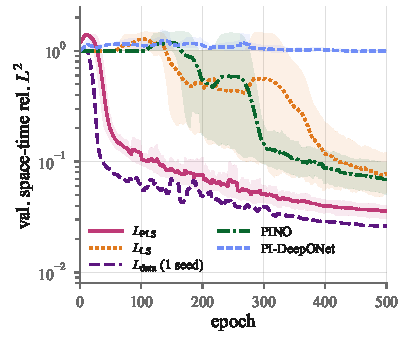
\includegraphics[width=0.49\linewidth]{figures/ac_val_curves.pdf}
  \hfill
  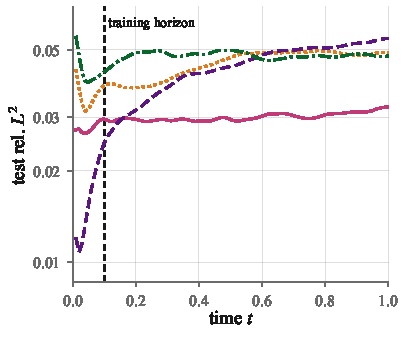
\includegraphics[width=0.49\linewidth]{figures/ac_long_rollout.pdf}
  \par\vspace{2pt}
  % One-row legend shared by both panels, authored at the full text width by plot_paper.py.
  
\includegraphics[width=\linewidth]{figures/ac_legend.pdf}
  \caption{Allen--Cahn. \textbf{Left:} validation space-time relative $L^2$ (pooled over the validation set) vs.\ epoch; mean over three seeds with min--max band, smoothed by a centered 15-epoch moving average. \textbf{Right:} test relative $L^2$ per time step of a free roll-out to $T=1$, mean over test samples of the per-sample error, for the best seed of each loss (selected on validation); PI-DeepONet, whose error stays between $0.7$ and $1$, is omitted. The dashed line marks the training horizon $t=0.1$.}
  \label{fig:ac-results}
\end{figure}

\subsubsection{Discussion}



\subsection{Stokes Equation}
Finally, we learn the solution operator $\mathcal G: f \mapsto (u, p)$ of the stationary Stokes equations
\begin{align}\label{eq:stokes_equation}
   \begin{split}
      -\mu\Delta u + \nabla p &= f, \qquad \nabla\cdot u = 0 \quad \text{in } \Omega,
      \\
      u &= 0 \quad \text{on } \partial\Omega, \qquad \textstyle\int_\Omega p\,\mathrm dx = 0,
   \end{split}
\end{align}
with $\mu = 1$ and the same family of sine-series body forces as in the Poisson experiment ($K = 10$). Two things change with respect to the previous two experiments, and they are the point of this one. First, the system is a \emph{saddle point}: the assembled $\mathcal K$ is symmetric but indefinite, so the Hessian of the bare least-squares loss is $\mathcal K^2$ with $\kappa = \mathcal O(h^{-4})$, and no block-diagonal operator approximates $\mathcal K^{-1}$. Following Section~\ref{sec:block_diagonal_preconditioner} we therefore use the block-diagonal $\mathcal P = \mathrm{diag}(\hat A^{-1}, \hat S^{-1})$ as the \emph{weighting matrix} of the loss, $L_{\textup{PLS}} = \tfrac12\,\mathbf r^\top \mathcal P\, \mathbf r$, for which $\kappa(\mathcal K \mathcal P \mathcal K) = \mathcal O(h^{-2})$. Second, $\Omega$ is \emph{not} a product domain: it is the unit square with a circular hole of radius $0.14$ centred at $(0.40, 0.50)$, with no-slip imposed on both components of $\partial\Omega$, discretized by an unstructured Taylor--Hood $P_2/P_1$ triangulation with $3998$ velocity and $1035$ pressure nodes ($9031$ degrees of freedom), matched in size to the $65^2/33^2$ grids of the Poisson experiment.

\textbf{Nothing in the loss depends on the domain being a grid.} The finite element residual $\mathcal K\mathbf c - \mathbf b$ is assembled from the mesh whatever the mesh is, so \eqref{eq:preconditiones_least_squares_loss} carries over verbatim; what has to be replaced are the two components that were grid-bound. The neural operator becomes GAOT [], which encodes the node values onto a fixed latent token grid, runs a transformer there and decodes back at the mesh nodes, so that the architecture never sees a physical grid; and the velocity block $\hat A^{-1}$ of $\mathcal P$ becomes one \emph{algebraic} multigrid V-cycle, built from the assembled stiffness matrix rather than from a hierarchy of nested grids. Both substitutions are internal to the method: the loss, the residual and the reference are untouched. Appendix~\ref{appendix:details_stokes} collects the mesh, the backbone and the selected hyperparameters.

\textbf{The preconditioner is what makes the saddle point trainable, and its Schur weight must be selected.} The bare least-squares loss $L_\textup{LS} = \tfrac12\|\mathcal K \mathbf c - \mathbf b\|^2$, our negative control, reaches $30.6 \pm 1.6\%$ velocity and $11.4 \pm 0.9\%$ pressure error at this budget, against $1.55\%$ / $0.85\%$ for $L_\textup{PLS}$ --- a factor of twenty, from weighting the same residual. Its error is also qualitatively different: smooth, large-scale and concentrated on the velocity maxima, the low-frequency modes that an $\mathcal O(h^{-4})$ objective releases last, whereas the preconditioned arm is at mesh-scale grain, i.e.\ at discretization level. The one free parameter of $\mathcal P$ is the Schur weight $\omega_S$, which sets the weight of the continuity rows relative to the momentum rows; it is selected on the validation set like a learning rate and has a broad optimum over $\omega_S \in [4, 16]$, degrading to $4.3\%$ at $\omega_S = 64$ and $22.9\%$ at $\omega_S = 256$ as the loss becomes pressure-dominated and the velocity loses the jets past the obstacle (Appendix~\ref{appendix:details_stokes}).

\textbf{The label-free loss surpasses supervised training by a factor of two.} Table~\ref{tab:summary} reports $1.55 \pm 0.20\%$ / $0.85 \pm 0.04\%$ for $L_\textup{PLS}$ against $3.27 \pm 0.15\%$ / $1.79 \pm 0.16\%$ for supervised training, with non-overlapping seed ranges on both fields and a comparable cost per epoch. Both arms target the same discrete Taylor--Hood state --- one through labels, the other through the residual whose zero it is --- so this says that the preconditioned residual is the better-conditioned route to that state, not that it solves an easier problem. This reverses the ordering of the previous two experiments, where $L_\textup{PLS}$ matched supervised training to within the seed spread on Poisson and trailed it on Allen--Cahn: on a geometry that no grid resolves, the label-free loss is ahead by a factor of two. PI-DeepONet, which differentiates the strong form by automatic differentiation through its coordinate trunk and therefore transfers to an arbitrary mesh, does not train on the saddle point and ends at $44\%$ / $35\%$.

\section{Conclusion}


%Citations within the text should be based on the \texttt{natbib} package
%and include the authors' last names and year (with the ``et~al.'' construct
%for more than two authors). When the authors or the publication are
%included in the sentence, the citation should not be in parenthesis using \verb|\citet{}| (as
%in ``See \citet{Hinton06} for more information.''). Otherwise, the citation
%should be in parenthesis using \verb|\citep{}| (as in ``Deep learning shows promise to make progress
%towards AI~\citep{Bengio+chapter2007}.'').

%The corresponding references are to be listed in alphabetical order of
%authors, in the \textsc{References} section. As to the format of the
%references themselves, any style is acceptable as long as it is used
%consistently.



\subsection*{AI use statement}

(This section is \textbf{required} and does not count toward the page limit.)

In this work, we used generative AI tools for software implementation and language refinement.
We have not used generative AI tools for drafting the manuscript,
and [the rest of the required disclosure tasks] are not applicable to this work.
Additionally, we used generative AI tools for [tasks with recommended
disclosure]. We have reviewed all AI-assisted work. LLM-generated code was verified and tested for correctness
by the authors. We take responsibility for the final content of this work,
including text, claims or artifacts produced with the aid of generative AI.


\subsection*{Ethics statement}

(This section is \textbf{recommended} and does not count toward the page limit.)

If authors feel that their paper submission raises questions regarding the Code
of Ethics, they are encouraged to include a paragraph of Ethics Statement (at
the end of the main text before references) to address potential concerns where
appropriate. Topics include, but are not limited to, studies that involve human
subjects, practices to data set releases, potentially harmful insights,
methodologies and applications, potential conflicts of interest and sponsorship,
discrimination/bias/fairness concerns, privacy and security issues, legal
compliance, and research integrity issues (e.g., IRB, documentation, research
ethics). This statement should not be more than 1 page.

\subsection*{Reproducibility statement}

(This section is \textbf{recommended} and does not count toward the page limit.)

It is important that the work published in ICLR is reproducible. Authors are
strongly encouraged to include a paragraph-long Reproducibility Statement at the
end of the main text (before references) to discuss the efforts that have been
made to ensure reproducibility. This paragraph should not itself describe
details needed for reproducing the results, but rather reference the parts of
the main paper, appendix, and supplemental materials that will help with
reproducibility. For example, for novel models or algorithms, a link to an
anonymous downloadable source code can be submitted as supplementary materials;
for theoretical results, clear explanations of any assumptions and a complete
proof of the claims can be included in the appendix; for any datasets used in
the experiments, a complete description of the data processing steps can be
provided in the supplementary materials. Each of the above are examples of
things that can be referenced in the reproducibility statement.

\subsubsection*{Author Contributions}
If you'd like to, you may include  a section for author contributions as is done
in many journals. This is optional and at the discretion of the authors.

\subsubsection*{Acknowledgments}
Use unnumbered third level headings for the acknowledgments. All
acknowledgments, including those to funding agencies, go at the end of the paper.


\bibliography{iclr2027_conference}
\bibliographystyle{iclr2027_conference}

\appendix
\section{Interpolated Neural Operators}
In this section, we explain why the form
\begin{equation*}
   \mathcal G_\theta(\rho) 
   =
   \sum_{i=1}^n\mathbf u(\theta, \rho)_i\,\phi_i
\end{equation*}
of \eqref{eq:neural_operator_interpolated_form} is not an essential restriction on the neural operator architecture. This simple observation is crucial for combining finite element tools with the flexibility of neural operators. Let us denote a neural operator parametrized by $\theta\in\Theta\cong \mathbb R^D$ by
\begin{equation*}
   \mathcal G_\theta:\mathcal P \to \mathcal U, \quad \rho \mapsto u = \mathcal G_\theta(\rho).
\end{equation*}
On this level $\mathcal G_\theta$ is abstract and maps functions to functions. For a given finite-dimensional subspace $\mathcal U_h\subset \mathcal U$ spanned by the basis $\phi_1,\dots,\phi_n$ and an \emph{interpolation operator}
\begin{equation*}
   \mathcal I_h : \mathcal U \to \mathcal U_h, \quad u\mapsto \mathcal I_h(u)
\end{equation*}
we can write $\mathcal I_h(u)$ in terms of the basis as
\begin{equation*}
   \mathcal I_h(u)
   =
   \sum_{i=1}^n \mathbf u_i\phi_i.
\end{equation*}
To obtain the interpolated neural operator form, we compose $\mathcal G_\theta$ with $\mathcal I_h$
\begin{equation}\label{eq:appendix_interpolated_form}
   [\mathcal I_h \circ \mathcal G_\theta](\rho)
   =
   \sum_{i=1}^n \mathbf u(\theta, \rho)_i \phi_i.
\end{equation}
Let $\mathcal G:\mathcal P\to\mathcal U$ denote the operator we wish to approximate and write $u = \mathcal G(\rho)$ for the exact solution. Assume that $\mathcal I_h$ is linear and stable, i.e., $\|\mathcal I_h(u)\|\leq C_{\mathcal I}\|u\|$ for all $u\in\mathcal U$. Adding and subtracting $\mathcal I_h(u)$ then gives, for every $\rho\in\mathcal P$,
\begin{align}\label{eq:appendix_interpolation_estimate}
   \begin{split}
      \big\| \mathcal G(\rho) - [\mathcal I_h\circ\mathcal G_\theta](\rho) \big\|
      &\leq
      \big\| u - \mathcal I_h(u) \big\|
      +
      \big\| \mathcal I_h\big(u - \mathcal G_\theta(\rho)\big) \big\|
      \\
      &\leq
      \big\| u - \mathcal I_h(u) \big\|
      +
      C_{\mathcal I}\,\big\| \mathcal G(\rho) - \mathcal G_\theta(\rho) \big\|.
   \end{split}
\end{align}
The interpolated operator is thus as accurate as the neural operator itself, up to the stability constant $C_{\mathcal I}$ and the interpolation error of the exact solution.

\paragraph{Example: the FNO} The FNO returns values on a uniform grid and for the space $\mathcal U_h = Q_1^h$ of our experiments the basis functions satisfy $\phi_i(x_j) = \delta_{ij}$, so the coefficients of the interpolant are precisely the point values, $\mathbf u(\theta,\rho)_i = [\mathcal G_\theta(\rho)](x_i)$. If in addition the FNO grid coincides with the nodes $x_1,\dots,x_n$, the interpolation is the identity in coordinates: $\mathcal I_h$ attaches the basis functions to the entries of the network's output array. For homogeneous Dirichlet boundary values, the basis spans the interior nodes only and $\mathcal I_h$ discards the values on $\partial\Omega$.


Interpolating a neural operator can be viewed as part of its architectural design, in which $\mathcal I_h$ acts as a problem-adapted, non-trainable output layer. By \eqref{eq:appendix_interpolation_estimate}, however, its accuracy cannot fall below the interpolation error $\| u - \mathcal I_h(u) \|$.

\section{Details of the Poisson Equation Experiment}\label{appendix:details_poisson}

\paragraph{Operator} We consider the Poisson equation with homogeneous Dirichlet boundary conditions on the unit square $\Omega = [0,1]^2$,
\begin{equation}\label{eq:appendix_poisson}
   -\Delta u = f \quad \text{in } \Omega, \qquad u = 0 \quad \text{on } \partial\Omega.
\end{equation}
For every $f\in H^{1}_0(\Omega)^*$ the Poisson equation admits a unique weak solution $u\in H^1_0(\Omega)$. We learn the associated solution operator 
\begin{equation*}
   \mathcal G: \mathcal F \to \mathcal U, \quad f \mapsto u,
\end{equation*}
with $\mathcal U = H^1_0(\Omega)$ and $\mathcal F=\mathcal U^*$. Hence $\mathcal G$ is the inverse of the Laplace operator.

\paragraph{Data Set} The dataset pairs $(f, u)$ are constructed through the eigenfunctions of the Laplacian, hence require no PDE solve. We draw coefficients $a_{ij}\sim\mathrm{Unif}[-1,1]$, independently for $i,j=1,\dots,K$, and set
\begin{align}\label{eq:appendix_poisson_data}
   \begin{split}
      f(x,y) &= \frac{\pi}{K^2}\sum_{i,j=1}^{K} a_{ij}\,(i^2+j^2)^{1/2}\,\sin(\pi i x)\sin(\pi j y),
      \\
      u(x,y) &= \frac{1}{\pi K^2}\sum_{i,j=1}^{K} a_{ij}\,(i^2+j^2)^{-1/2}\,\sin(\pi i x)\sin(\pi j y).
   \end{split}
\end{align}
The pairs satisfy $-\Delta u = f$ exactly and vanish at the boundary. The parameter $K$ controls the amount of frequencies in the data, and a larger $K$ constitutes a more challenging learning problem. Figure~\ref{fig:poisson_dataset} shows one draw at each value.

\begin{figure}[htb]
   \centering
   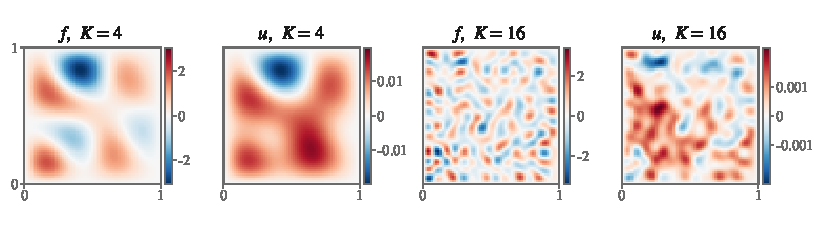
\includegraphics[width=\linewidth]{figures/poisson_dataset_samples.pdf}
   \caption{Samples from the Poisson data set, drawn from \eqref{eq:appendix_poisson_data} on a $65^2$ grid: source and solution at $K=4$ (left pair) and at $K=10$ (right pair). Note the differing magnitudes of $u$.}
   \label{fig:poisson_dataset}
\end{figure}

\paragraph{Discretization} We partition $\Omega$ into a uniform grid of $(n_x-1)^2$ squares with mesh size $h = 1/(n_x-1)$, and approximate in the space of continuous, piecewise \emph{bilinear} finite elements
\begin{equation*}
   \mathcal U_h = Q_1^h = \big\{ v \in C(\overline\Omega) \;:\; v|_T \in \operatorname{span}\{1, x, y, xy\} \text{ for every cell } T, \quad v|_{\partial\Omega} = 0 \big\}.
\end{equation*}
We write $\phi_1, \dots, \phi_n$ for the associated global basis functions that are characterized through $\phi_i(x_j) = \delta_{ij}$ on the interior grid nodes $x_1, \dots, x_n$. This means that $n = \dim \mathcal U_h = (n_x-2)^2$. We use $n_x = 65$, hence $n = 3969$. The stiffness and mass matrices are
\begin{equation}\label{eq:appendix_stiffness_mass}
   A_{ij} = \int_\Omega \nabla\phi_j \cdot \nabla\phi_i \,\mathrm dx,
   \qquad
   M_{ij} = \int_\Omega \phi_j\,\phi_i \,\mathrm dx,
\end{equation}
which we assemble with an exact quadrature rule. For the analytical sources $f$ we use its \emph{nodal approximation}, i.e., we replace $f$ by its interpolant $\sum_{j=1}^n f(x_j)\phi_j \in \mathcal U_h$. The discretized forcing thus becomes
\begin{equation}\label{eq:appendix_consistent_rhs}
   \mathbf f_i = \sum_{j=1}^n M_{ij}\,f(x_j).
\end{equation}

\paragraph{Neural Operator} We use a FNO as implemented in the \texttt{neuraloperator} package []. The hyperparameters are collected in Table~\ref{tab:fno}. Because the FNO grid coincides with the finite element nodes, the interpolation into $\mathcal U_h$ of \eqref{eq:neural_operator_interpolated_form} is the identity. Zero boundary conditions are hard-enforced by projecting to zero on $\partial\Omega$, so the model output lies in $\mathcal U_h$ exactly.

\paragraph{Baselines} PINO [] and PI-DeepONet [] are the two published label-free approaches we compare against. Both minimize the \emph{strong-form} residual $-\Delta u - f$ at the interior grid nodes, reduced as the relative ratio $\|{-\Delta_h u} - f\|_2 / \|f\|_2$ of the reference implementation, and they differ in how the Laplacian is obtained: PINO uses the FNO of Table~\ref{tab:fno} with second-order central differences on the grid (the \texttt{FiniteDiff} utility of the reference library), whereas PI-DeepONet uses an unstacked DeepONet ($p=128$ basis functions, branch and trunk MLPs of width $256$ and depth $4$, $64$ random Fourier features on the trunk input, $1.4\cdot 10^6$ parameters) differentiated exactly by automatic differentiation through the coordinate input of the trunk. The two residuals are the same PDE at the same accuracy: evaluated at the analytical solution they agree to $0.7\%$, and both converge at second order. We impose the boundary condition on both baselines exactly as on our own arms, by setting the boundary nodes of the output to zero. The reference implementations instead multiply the output by the ansatz $\sin(\pi x)\sin(\pi y)$, which on the present data set, a truncated sine series, encodes much of the structure of the solution and does not transfer to other geometries; we therefore report it only as a control. For PINO the zeroed boundary ring enters the residual through the finite-difference stencil, whereas a pointwise autodiff Laplacian cannot see a mask, so PI-DeepONet additionally carries the soft boundary penalty of the original formulation, $\lambda_{\mathrm{bc}}$ times the root-mean-square of the prediction on $\partial\Omega$ relative to its root-mean-square in the interior; without it the objective is invariant under the addition of harmonic functions, and the relative error exceeds $160\%$. With the ansatz PI-DeepONet reaches $0.191 \pm 0.005$ instead of the $0.214 \pm 0.047$ of Table~\ref{tab:summary}. Its seed-to-seed spread, $0.163$ to $0.258$, is the largest in the table, and every baseline run is still descending at the end of the budget, so these numbers characterize the fixed budget rather than a converged state.

\begin{table}[htb]
   \caption{FNO hyperparameters used for all Poisson experiments.}
   \label{tab:fno}
   \begin{center}
   \begin{tabular}{ll}
      \multicolumn{1}{c}{\bf Component} & \multicolumn{1}{c}{\bf Value} \\ \hline \\
      Fourier modes.             & $16\times16$ \\
      Hidden channels (width)    & $64$ \\
      Fourier layers             & $5$ \\
      Lifting / projection channels & $128$ / $128$ \\
      Positional embedding       & grid coordinates, appended as channels \\
      Input / output channels    & $1$ / $1$ \\
      Trainable parameters       & $3.01\times10^{6}$ \\
   \end{tabular}
   \end{center}
\end{table}

\paragraph{Multigrid Preconditioner} We take $P$ to be a single geometric multigrid V-cycle for $A$ starting from a zero initial guess. We use dyadic coarsening on grids of fineness $2^k+1$ to guarantee nested grids, and denote by $A_\ell$ the stiffness matrix on level $\ell=0,\dots,L-1$, where $\ell=0$ is the finest grid and $L$ the number of levels. As smoother, we use weighted Jacobi with $\nu_1=\nu_2=2$ iterations and damping $\omega=8/9$, which is the optimal value for $Q_1$ elements in two dimensions, bilinear prolongation $\Pi_\ell$ with restriction $\Pi_\ell^\top$, and a direct solve on the coarsest grid; Algorithm~\ref{alg:vcycle} summarizes the V-cycle.

\begin{algorithm}[htb]
   \caption{V-cycle $\mathrm{V}(\ell,\mathbf r)$ on level $\ell$; the preconditioner is $P\mathbf r := \mathrm{V}(0,\mathbf r)$. Here $D_\ell = \operatorname{diag}(A_\ell)$.}
   \label{alg:vcycle}
   \begin{algorithmic}[1]
      \If{$\ell = L-1$}
         \State \Return $A_{L-1}^{-1}\mathbf r$ \Comment{coarsest grid: direct solve}
      \EndIf
      \State $\mathbf e \gets \mathbf 0$
      \For{$\nu_1$ sweeps}
         \State $\mathbf e \gets \mathbf e + \omega\, D_\ell^{-1}\big(\mathbf r - A_\ell \mathbf e\big)$ \Comment{pre-smoothing}
      \EndFor
      \State $\mathbf r_c \gets \Pi_\ell^\top\big(\mathbf r - A_\ell \mathbf e\big)$ \Comment{restrict the residual}
      \State $\mathbf e \gets \mathbf e + \Pi_\ell\, \mathrm{V}(\ell+1, \mathbf r_c)$ \Comment{coarse-grid correction}
      \For{$\nu_2$ sweeps}
         \State $\mathbf e \gets \mathbf e + \omega\, D_\ell^{-1}\big(\mathbf r - A_\ell \mathbf e\big)$ \Comment{post-smoothing}
      \EndFor
      \State \Return $\mathbf e$
   \end{algorithmic}
\end{algorithm}

\paragraph{Optimization} The FNO is trained with Adam and a cosine annealed learning rate; see Table~\ref{tab:optim}. Every setting is shared across losses and preconditioners \emph{except the learning rate}, which is tuned per loss. The rate is selected by a grid search over $\{10^{-4}, 3\cdot 10^{-4}, 10^{-3}, 3\cdot 10^{-3}, 10^{-2}, 3\cdot 10^{-2}\}$, run at the full $500$-epoch budget with a single seed, choosing the rate that attains the lowest validation relative $L^2$ over training. For PI-DeepONet, whose boundary penalty introduces a second hyperparameter, the weight $\lambda_{\mathrm{bc}}$ is tuned jointly with the learning rate on the grid $\{3\cdot 10^{-5}, 10^{-4}, 3\cdot 10^{-4}, 10^{-3}\} \times \{0.3, 1, 3\}$, extended to $\lambda_{\mathrm{bc}} \in \{0.1, 0.03, 0.01, 0.003, 0.001, 0\}$ at the best rates whenever the optimum fell on the edge of the grid; the selected pair $(10^{-4}, 0.03)$ is an interior optimum in both variables, with the validation error rising to $0.24$ at $\lambda_{\mathrm{bc}}=0.01$ and $0.30$ at $0.1$. The final runs then repeat the selected configuration over three seeds. Throughout, the checkpoint attaining the lowest validation error is restored after training, and the reported test error is evaluated at that checkpoint.

\begin{table}[htb]
   \caption{Optimization hyperparameters for the Poisson experiments. Shared across losses except
   the learning rate, which is swept per loss as described above.}
   \label{tab:optim}
   \begin{center}
   \begin{tabular}{ll}
      \multicolumn{1}{c}{\bf Setting} & \multicolumn{1}{c}{\bf Value} \\ \hline \\
      Optimizer                 & Adam, $\beta_1 = 0.9$, $\beta_2 = 0.999$, $\varepsilon = 10^{-8}$ \\
      Weight decay              & $0$ \\
      Schedule                  & cosine, annealed from $\eta$ to $\eta/10$ over all epochs \\
      Learning rate $\eta$      & $3\cdot 10^{-4}$ for $L_\textup{data}$ and $L_\textup{PLS}$ \\
                                & $3\cdot 10^{-3}$ for $L_\textup{LS}$ and PINO \\
                                & $10^{-4}$ for PI-DeepONet, with boundary penalty weight $\lambda_{\mathrm{bc}} = 0.03$ \\
      Epochs                    & $500$ \\
      Batch size                & $32$ \\
      Train / validation / test samples & $1024$ / $128$ / $256$ \\
      Model selection           & lowest validation relative $L^2$, restored after training \\
      Random seeds              & $42, 43, 44$ (final runs); $42$ for the learning-rate sweep \\
   \end{tabular}
   \end{center}
\end{table}

\section{Details of the Stokes Equation Experiment}\label{appendix:details_stokes}

\paragraph{Operator} We consider the stationary Stokes equations \eqref{eq:stokes_equation} with viscosity $\mu = 1$ and learn the solution operator $\mathcal G: f \mapsto (u, p)$ from the body force to the velocity--pressure pair. In the weak form, $\mathcal U = H^1_0(\Omega)^2 \times L^2_0(\Omega)$ and $a\big((u,p),(v,q)\big) = \mu(\nabla u, \nabla v) - (p, \nabla\cdot v) - (q, \nabla\cdot u)$, a symmetric but indefinite bilinear form; this is the saddle point setting of Section~\ref{sec:block_diagonal_preconditioner}, and it is the reason the preconditioner enters the loss as a norm weight rather than as an approximate inverse.

\paragraph{Domain and Mesh} $\Omega$ is the unit square with a circular hole of radius $0.14$ centred at $(0.40, 0.50)$. The hole is placed off-centre deliberately, so that the solution does not inherit a symmetry of the domain, and the no-slip condition $u = 0$ is imposed on \emph{both} components of $\partial\Omega$. The mesh is an unstructured Gmsh triangulation at target edge length $0.035$, emitted as quadratic triangles, giving $1928$ elements, $3998$ velocity ($P_2$) nodes of which $284$ lie on $\partial\Omega$, and $1035$ pressure ($P_1$) nodes, i.e.\ $2\cdot 3998 + 1035 = 9031$ degrees of freedom with $568$ velocity components constrained. The size is chosen to match the $65^2 = 4225$ velocity and $33^2 = 1089$ pressure nodes of a structured Taylor--Hood grid at the same problem size, so that the dimension of the discrete problem and the cost of the model are comparable to the Poisson experiment rather than to a coarser one. The boundary node set is taken from the incidence of the boundary facet elements rather than from a coordinate predicate, which on a curved boundary misses nodes placed a rounding unit off the exact geometry.

\paragraph{Data Set} Each component of the body force is a truncated sine series with the same spectral decay as the Poisson sources,
\begin{equation}\label{eq:appendix_stokes_data}
   f_c(x,y) = \sum_{k,l=1}^{K} a_{ckl}\,(k^2+l^2)^{-1/2}\,\sin(k\pi x)\sin(l\pi y), \qquad c = 1, 2, \qquad a_{ckl} \sim \mathrm{Unif}[-1,1],
\end{equation}
with $K = 10$ as in the Poisson experiment. No closed-form solution exists; the reference $(u, p)$ is the \emph{discrete} Taylor--Hood solution of the system below, computed once per sample by a sparse direct solve in double precision with the pressure pinned at one node and subsequently re-gauged to zero mean, so that the label-free residual and the labels target the same discrete state. The factorization is shared across samples and the relative residual of the reference is $4.4\cdot 10^{-6}$. Stokes is linear, and we use the one free constant per sample to rescale $(f, u, p)$ so that the reference velocity has unit finite element $L^2$ norm. The physics then fixes the other two magnitudes, $u \sim f/(\mu k^2)$ and $p \sim f/k$: at unit velocity the nodal root-mean-square values are $\mathcal O(10^2)$ for $f$ and $\mathcal O(10)$ for $p$. The network therefore sees $f / f_{\mathrm{scale}}$, and its pressure channel is read as $p_{\mathrm{scale}}$ times the raw output; both are fixed constants of the data set applied at the network boundary, and neither the operator, the residual nor the reference sees them. Training, validation and test sets of $1024$, $128$ and $256$ samples are contiguous slices of one pool; as for Poisson, the seed draws both the pool and the initialization.

\paragraph{Discretization} We use the Taylor--Hood $P_2/P_1$ pair on the triangulation above: the velocity is continuous piecewise quadratic on all $3998$ nodes and the pressure continuous piecewise linear on the $1035$ vertices. Assembling the bilinear form gives the symmetric indefinite system
\begin{equation}\label{eq:appendix_stokes_system}
   \mathcal K \mathbf c = \begin{pmatrix} A & B^\top \\ B & 0 \end{pmatrix} \begin{pmatrix} \mathbf u \\ \mathbf p \end{pmatrix} = \begin{pmatrix} M_u \mathbf f \\ 0 \end{pmatrix},
\end{equation}
where $A = \mu\,\mathrm{diag}(A_{P_2}, A_{P_2})$ is the vector stiffness matrix, $B$ the discrete divergence, and $M_u \mathbf f$ the consistent load of the nodal interpolant of $f$. The residual is set to zero on the constrained velocity degrees of freedom, and for every arm --- at training and evaluation time alike --- the prediction is projected onto the admissible space: the velocity to zero on $\partial\Omega$ and the pressure to zero mean in the lumped $M_p$ inner product, since $B^\top \mathbf 1 = 0$ makes the residual blind to the constant pressure mode. We verify the assembly by probing $\mathcal K\,(\mathbf 0, \mathbf 1)$ on the free momentum rows: a self-consistent solve does \emph{not} detect a permuted quadratic element, whereas this probe does.

\paragraph{Neural Operator} A finite element residual needs only nodal values, but a Fourier neural operator needs an image, so on this mesh the backbone is the Geometry-Aware Operator Transformer (GAOT) [], with two input and three output channels $(u_x, u_y, p)$ and $3.40\cdot 10^{6}$ parameters --- within $13\%$ of the FNO used for Poisson and Allen--Cahn. It consists of a multiscale attentional kernel-integral encoder that lifts the nodal values onto a fixed structured grid of $64\times 64$ latent tokens, a vision-transformer processor on those tokens (patch size $2$, lifting width $64$, $3$ layers of width $256$), and a decoder of the same kernel-integral form that evaluates at the mesh nodes. The physical mesh therefore enters only through the encoder and decoder neighbourhoods, whose radius is set to $2.1\,\max(h_{\mathrm{phys}}, h_{\mathrm{latent}})$ so that a change of resolution can neither empty nor saturate the neighbour graph. We confirmed on the structured Poisson problem of Appendix~\ref{appendix:details_poisson}, where both backbones apply, that the ordering of the losses is a property of the objective and not of the architecture: over three seeds GAOT reaches $0.55\%$ against the FNO's $0.59\%$ for $L_\textup{data}$ and $0.61\%$ against $0.66\%$ for $L_\textup{PLS}$, with the bare least-squares control two orders of magnitude behind for both.

\paragraph{Preconditioner} We take the block-diagonal $\mathcal P = \mathrm{diag}(\hat A^{-1}, \hat S^{-1})$ of Section~\ref{sec:block_diagonal_preconditioner}. A geometric hierarchy does not exist on this mesh, so $\hat A^{-1}$ applies one \emph{algebraic} multigrid V$(2,2)$ cycle per velocity component, built by classical coarsening from the assembled $P_2$ stiffness matrix ($n = 3998$, $41166$ nonzeros, damped block-Jacobi smoothing) and divided by $\mu$; its measured contraction is about $0.4$ per cycle. $\hat S^{-1} = \omega_S\,\mu\,\mathrm{diag}(M_p)^{-1}$ is the lumped pressure mass matrix, the classical spectrally equivalent surrogate of the Schur complement, and is mesh-agnostic as it stands. Since no block-diagonal operator approximates $\mathcal K^{-1}$, $\mathcal P$ enters the least-squares loss as the weighting matrix $B$ of \eqref{eq:preconditiones_least_squares_loss}, $L_{\mathrm{PLS}}(\mathbf c) = \tfrac12\, (\mathcal K \mathbf c - \mathbf b)^\top \mathcal P (\mathcal K \mathbf c - \mathbf b)$, whose Hessian $\mathcal K \mathcal P \mathcal K$ has condition number $\mathcal O(h^{-2})$ instead of the $\mathcal O(h^{-4})$ of the bare residual. The monolithic multigrid alternative, a genuine $\mathcal P \approx \mathcal K^{-1}$, is not available here: its transfer operators are geometric, requiring both fields to nest by a factor of two on a grid.

\paragraph{Baseline} PI-DeepONet minimizes the strong form of \eqref{eq:stokes_equation} at interior collocation points, with the momentum and continuity residuals stacked into one relative ratio, $\|(r_{\mathrm{mom}}, w\, r_{\mathrm{div}})\|_2 / \|(f, 0)\|_2$. It is the physics-informed baseline that transfers to this setting: its derivatives are taken by automatic differentiation through the coordinate input of the trunk, which is defined at any point of $\Omega$, whereas a finite-difference residual presupposes a grid and has no counterpart on an unstructured mesh. We use a DeepONet with three output channels, $p = 128$ basis functions, branch and trunk of width $256$ and depth $4$, $64$ random Fourier features on the trunk input and $2.54\cdot 10^{6}$ parameters, with the sensor set taken to be the mesh nodes. The boundary condition is imposed on the velocity exactly as on our own arms, by setting the velocity at the boundary nodes to zero; because a pointwise autodiff Laplacian at an interior collocation point cannot see a mask on the boundary values, the loss additionally carries the relative boundary penalty $\lambda_{\mathrm{bc}}$ of the Poisson experiment, and without it the objective is invariant under the addition of harmonic fields. The $\sin(\pi x)\sin(\pi y)$ ansatz used by the reference implementation is not available on this domain, since no closed form vanishes on both components of $\partial\Omega$. The autodiff residual retains a second-order graph for three fields at every collocation point, so the loss is evaluated at $1024$ interior nodes drawn afresh at every step.

\paragraph{Optimization} The protocol is that of the Poisson experiment (Table~\ref{tab:optim}): Adam with a cosine schedule from $\eta$ to $\eta/10$ over $500$ epochs, batch size $32$, $1024$/$128$/$256$ samples, and for every arm a grid search at the full budget on seed $42$ selecting the configuration with the lowest validation error, followed by three seeds. The validation error, and hence the model selection, is the mean of the velocity and pressure relative errors. The Schur weight was searched over $\omega_S \in \{0.5, 4, 16, 32, 64, 256\}$ at $\eta = 10^{-3}$, and for PI-DeepONet the learning rate, boundary weight and continuity weight over the grid of the structured Poisson study, whose selected values $(\eta, \lambda_{\mathrm{bc}}, w) = (10^{-4}, 0.1, 100)$ were re-selected here; at that rate $w = 1$ gives $80.9\%$ and $w = 1000$ gives $100.0\%$. Table~\ref{tab:optim_stokes} lists the selected values.

\begin{table}[htb]
   \caption{Optimization hyperparameters for the Stokes experiment; everything not listed is as in Table~\ref{tab:optim}.}
   \label{tab:optim_stokes}
   \begin{center}
   \begin{tabular}{ll}
      \multicolumn{1}{c}{\bf Setting} & \multicolumn{1}{c}{\bf Value} \\ \hline \\
      Learning rate $\eta$      & $10^{-3}$ for $L_\textup{PLS}$, with Schur weight $\omega_S = 16$ \\
                                & $10^{-3}$ for $L_\textup{data}$ and $L_\textup{LS}$ \\
                                & $10^{-4}$ for PI-DeepONet, with $w = 100$ and $\lambda_{\mathrm{bc}} = 0.1$ \\
      Collocation (PI-DeepONet) & $1024$ interior nodes per step, resampled every step \\
      Model selection           & lowest validation mean of the velocity and pressure relative $L^2$ \\
      Preconditioner            & block; velocity half one algebraic V$(2,2)$ cycle \\
      Random seeds              & $42, 43, 44$ (final runs); $42$ for the grid search \\
   \end{tabular}
   \end{center}
\end{table}

\paragraph{Metric} Velocity and pressure are scored separately, each in its own finite element $L^2$ norm against the discrete reference, as the dataset-level relative error $\big(\sum_i \|e_i\|_M^2 / \sum_i \|c^*_i\|_M^2\big)^{1/2}$ with $M = M_u$ for the velocity and $M = M_p$ for the pressure, on the test set at the best-validation checkpoint; Table~\ref{tab:summary} reports both, each as mean $\pm$ half-range over the three seeds. The supervised and preconditioned arms are still improving at the end of the budget (best epoch $492$ and $498$ of $500$), so their numbers characterize the fixed budget rather than a converged state; the bare least-squares control is not, peaking between epochs $64$ and $77$ and drifting upwards thereafter.

\paragraph{Preconditioner ablation} Table~\ref{tab:stokes_ablation} isolates the contribution of $\mathcal P$ on the same mesh, budget and backbone. Removing it entirely costs a factor of twenty on the velocity. Keeping it but mis-weighting its pressure block is almost as damaging, and in a specific way: $\omega_S$ multiplies the pressure block of the norm the loss measures in, so a large $\omega_S$ makes that norm pressure-dominated and the optimizer serves the pressure at the velocity's expense. At $\omega_S = 256$ the pressure error is still $3.9\%$ while the velocity error is $22.9\%$, concentrated in a wake-shaped region behind the obstacle where the flow has lost its jets. The optimum is a broad plateau over $\omega_S \in [4, 16]$, and $\omega_S = 16$ is also the value that minimizes $\kappa(\mathcal K \mathcal P \mathcal K)$ for this operator.

\begin{table}[htb]
   \caption{Preconditioner ablation on the unstructured Stokes problem: test relative finite element $L^2$ error of velocity and pressure, seed $42$, everything else as in Table~\ref{tab:summary}. $L_\textup{LS}$ is the bare least-squares loss, i.e.\ $\mathcal P = I$.}
   \label{tab:stokes_ablation}
   \begin{center}
   \begin{tabular}{lcc}
      \multicolumn{1}{c}{\bf Loss} & \multicolumn{1}{c}{\bf velocity} & \multicolumn{1}{c}{\bf pressure} \\ \hline \\
      $L_\textup{LS}$ (no preconditioner)   & $30.5\%$ & $10.2\%$ \\
      $L_\textup{PLS}$, $\omega_S = 0.5$    & $2.58\%$ & $1.25\%$ \\
      $L_\textup{PLS}$, $\omega_S = 4$      & $1.63\%$ & $0.95\%$ \\
      $L_\textup{PLS}$, $\omega_S = 16$     & $1.69\%$ & $0.79\%$ \\
      $L_\textup{PLS}$, $\omega_S = 32$     & $3.35\%$ & $1.40\%$ \\
      $L_\textup{PLS}$, $\omega_S = 64$     & $4.25\%$ & $1.62\%$ \\
      $L_\textup{PLS}$, $\omega_S = 256$    & $22.94\%$ & $3.93\%$ \\
   \end{tabular}
   \end{center}
\end{table}

\section{Details of the Allen--Cahn Experiment}\label{appendix:details_allen_cahn}

\paragraph{Operator} We consider the Allen--Cahn equation with homogeneous Dirichlet boundary conditions on the unit square $\Omega = [0,1]^2$ and the time interval $I = [0,T]$,
\begin{equation}\label{eq:appendix_allen_cahn}
   \partial_t u - \Delta u + \varepsilon^2\big(u^3 - u\big) = 0 \quad \text{in } I\times\Omega,
   \qquad
   u = 0 \quad \text{on } I\times\partial\Omega,
   \qquad
   u(0) = u_0 \quad \text{in } \Omega.
\end{equation}
The Allen--Cahn equation is the $L^2(\Omega)$ gradient flow $\partial_t u = -E'(u)$ of the Ginzburg--Landau energy
\begin{equation}\label{eq:appendix_ginzburg_landau}
   E(u) = \frac12\int_\Omega |\nabla u|^2\,\mathrm dx + \frac{\varepsilon^2}{4}\int_\Omega \big(u^2 - 1\big)^2\,\mathrm dx,
\end{equation}
hence $t\mapsto E(u(t))$ is non-increasing. The double-well potential drives $u$ towards the two phases $u = \pm 1$, which are separated by interfaces of width $\mathcal O(\varepsilon^{-1})$; we use $\varepsilon = 32$. For every $u_0\in L^2(\Omega)$, \eqref{eq:appendix_allen_cahn} admits a unique weak solution
\begin{equation*}
   u \in L^2(I;H^1_0(\Omega)) \cap L^4(I\times\Omega) \cap C(I;L^2(\Omega)),
   \qquad
   \partial_t u \in L^2(I;H^{-1}(\Omega)) + L^{4/3}(I\times\Omega),
\end{equation*}
by the theory of monotone operators: $u\mapsto -\Delta u + \varepsilon^2 u^3$ is monotone and $u\mapsto -\varepsilon^2 u$ is a Lipschitz perturbation, see []. The initial conditions we use satisfy $\|u_0\|_{L^\infty(\Omega)} \leq 0.96$, see the data set description below, and by the maximum principle the solution then satisfies $\|u(t)\|_{L^\infty(\Omega)}\leq 1$ for all $t\in I$. The cubic term is therefore bounded along all trajectories we consider, and the solutions lie in the standard energy space
\begin{equation*}
   W(I) = \big\{ u\in L^2(I;H^1_0(\Omega)) \;:\; \partial_t u \in L^2(I;H^{-1}(\Omega)) \big\} \hookrightarrow C(I;L^2(\Omega)).
\end{equation*}
We denote by $S(t)u_0 = u(t)$ the solution semigroup on $L^2(\Omega)$. Testing the difference of two solutions with itself, and using that $u\mapsto u^3$ is monotone and that $2\pi^2$ is the smallest eigenvalue of $-\Delta$ on $\Omega$, yields
\begin{equation}\label{eq:appendix_ac_stability}
   \|S(t)u_0 - S(t)v_0\|_{L^2(\Omega)} \leq e^{(\varepsilon^2 - 2\pi^2)\,t}\,\|u_0 - v_0\|_{L^2(\Omega)}.
\end{equation}
The exponential factor is not an artifact of the estimate: linearizing \eqref{eq:appendix_allen_cahn} at the unstable equilibrium $u = 0$ shows that the mode $\sin(\pi i x)\sin(\pi j y)$ grows at rate $\varepsilon^2 - \pi^2(i^2 + j^2)$, which is the mechanism behind phase separation. Perturbations of an early, small-amplitude state are hence strongly amplified, which is relevant for autoregressive rollouts. Rather than approximating $S(t)$ directly, we learn a time-discrete approximation of $S(\tau)$ for a fixed time step $\tau > 0$, which we define next.

\paragraph{Time Discretization} We split the energy into two convex parts, $E = E_+ - E_-$, with
\begin{equation*}
   E_+(u) = \frac12\int_\Omega |\nabla u|^2\,\mathrm dx + \frac{\varepsilon^2}{4}\int_\Omega \big(u^4 + 1\big)\,\mathrm dx,
   \qquad
   E_-(u) = \frac{\varepsilon^2}{2}\int_\Omega u^2\,\mathrm dx,
\end{equation*}
and discretize the gradient flow with the convex--concave splitting of [], which treats $E_+$ implicitly and $E_-$ explicitly. Given $u_k \in L^2(\Omega)$, the next time step $u_{k+1}\in H^1_0(\Omega)$ solves
\begin{equation}\label{eq:appendix_cc_step}
   \frac1\tau\big(u_{k+1} - u_k, v\big) + \big(\nabla u_{k+1}, \nabla v\big) + \varepsilon^2\big(u_{k+1}^3 - u_k, v\big) = 0
   \quad \text{for all } v\in H^1_0(\Omega),
\end{equation}
where $(\cdot,\cdot)$ denotes the $L^2(\Omega)$ inner product. Equivalently, $u_{k+1}$ is the minimizer of
\begin{equation}\label{eq:appendix_cc_functional}
   J(v; u_k) = E_+(v) - \varepsilon^2 (u_k, v) + \frac{1}{2\tau}\|v - u_k\|^2_{L^2(\Omega)},
   \qquad v \in H^1_0(\Omega),
\end{equation}
and \eqref{eq:appendix_cc_step} is its Euler--Lagrange equation. As $H^1_0(\Omega)\hookrightarrow L^4(\Omega)$ in two dimensions, $J(\cdot\,; u_k)$ is finite, strictly convex, coercive and weakly lower semicontinuous on $H^1_0(\Omega)$. It thus has a unique minimizer for every $u_k\in L^2(\Omega)$ and every $\tau > 0$, and the scheme is well defined without a step size restriction. It is moreover unconditionally energy stable: for $u_k\in H^1_0(\Omega)$, convexity of $E_+$ at $u_{k+1}$ and of $E_-$ at $u_k$ gives
\begin{equation*}
   E(u_{k+1}) - E(u_k)
   \leq
   \big\langle E_+'(u_{k+1}) - E_-'(u_k),\, u_{k+1} - u_k \big\rangle
   =
   -\frac1\tau\|u_{k+1} - u_k\|^2_{L^2(\Omega)},
\end{equation*}
where the equality is \eqref{eq:appendix_cc_step} tested with $v = u_{k+1} - u_k$. The operator we learn is the resulting time-stepping operator
\begin{equation*}
   \mathcal G_\tau : L^2(\Omega) \to H^1_0(\Omega), \quad u_k \mapsto u_{k+1},
\end{equation*}
whose iterates $\mathcal G_\tau^k(u_0)$ are a first-order approximation in $\tau$ of $u(k\tau) = S(k\tau)u_0$. For the loss functions it is convenient to characterize $\mathcal G_\tau$ through the residual $\Phi : H^1_0(\Omega)\times L^2(\Omega) \to H^{-1}(\Omega)$, defined by
\begin{equation}\label{eq:appendix_cc_residual}
   \big\langle \Phi(w, u_k), v \big\rangle
   =
   \frac1\tau\big(w - u_k, v\big) + \big(\nabla w, \nabla v\big) + \varepsilon^2\big(w^3 - u_k, v\big)
   \quad \text{for all } v\in H^1_0(\Omega),
\end{equation}
so that $\Phi(\cdot, u_k) = D_v J(\cdot\,; u_k)$ and $\mathcal G_\tau(u_k)$ is the unique root of $\Phi(\cdot, u_k)$. Restricting $w$ and $v$ in \eqref{eq:appendix_cc_residual} to $\mathcal U_h = Q_1^h$, and replacing $w^3$ by its nodal interpolant, yields the discrete residual $\phi$ of \eqref{eq:convex_concave_time_stepper}.

\end{document}
